\chapter{Solving Linear Systems}
\label{ch:ch3}

\section{Linear Systems}

\subsection{General Form of Linear Systems}

So far, we have seen systems of linear equations as the equations that
describe points, lines and planes. However, linear systems of
equations show up in many other ways in engineering problems. We will
solve linear systems to find the behaviour of an electrical circuit. 
Other examples
would be the calculation of equilibrium temperature distributions or
electric fields. Such examples often involve the discretization of a
continuous function. In other words, a continuous function like the
temperature distribution in a body (which has a value for each of the
infinitely many points in the body) will be replaced by a list of
temperatures at a large but finite number $n$ of closely spaced
points. This gives rise to a system of linear equations in $n$
unknowns, where $n$ can be in the tens of thousands, or
higher. Therefore, we want to develop a technique to solve systems of
linear equations in $n$ unknowns when $n$ is large.

The most general form of a linear system of equations is
\[
\matrix{
a_{1,1}x_1  &+&a_{1,2}x_2   &+\cdots    &+&a_{1,n}x_n   &= &c_1\cr
a_{2,1}x_1  &+&a_{2,2}x_2   &+\cdots    &+&a_{2,n}x_n   &= &c_2\cr
\vdots      &\vdots&        &   &&\vdots        &&\vdots\cr
a_{m,1}x_1  &+&a_{m,2}x_2   &+\cdots    &+&a_{m,n}x_n   &= &c_m\cr
}
\]
Here the numbers $a_{i,j}$ and $c_j$ are known, and the goal is to find
all values of $x_1,\ldots ,x_n$ that satisfy all the equations.

\subsection{Solving Linear Systems by Substitution}

Let us start with an example, which we will solve using the method of
{\em substitution}.
\begin{example}
\label{ex_substitution}
Consider the system of equations
\[\matrix{
x_1&+&x_2&+&x_3&=&6\cr
x_1&-&x_2&+&x_3&=&0\cr
2x_1&+&x_2&-&8x_3&=&-11\cr
}
\]
{\rm One could try to proceed as follows. Solve the first equations
for, say, $x_3$. This gives
\[
x_3=6-x_1-x_2.
\]
Now substitute this value for $x_3$ into the second and third equations.
This gives
\[
\matrix{
x_1&-&x_2&+&(6-x_1-x_2)&=&0\cr
2x_1&+&x_2&-&8(6-x_1-x_2)&=&-11\cr
}
\]
or
\begin{eqnarray*}
-2x_2 &=& -6 \\
10x_1+9x_2 &=& 37
\end{eqnarray*}
Now solve the first of these equations for $x_2$ and substitute into
the last equation. This gives $x_2=3$ and $x_1=1$. Finally we can go
back and calculate $x_3=6-1-3=2$.}
\end{example}

Although this procedure works fine for $n=2$ or even $n=3$, it rapidly
becomes unwieldy for larger values of $n$. We will now introduce a
technique called Gaussian elimination that works well for large $n$
and can be easily implemented on a computer.

We have already observed that there may be many systems of equations
with the same solution. When there are only two unknowns, this amounts
to saying that different pairs of lines may intersect in the same
point.  Gaussian elimination is based on the following idea.  We
introduce three elementary row operations. These operations change the
system of the equations into another system with exactly the same the
set of solutions. We then apply these elementary row operations in a
systematic way to change the system of equations into a system that is
easily solved.

\subsection{Elementary row (equation) operations}

The first elementary row operation is

\vspace{2mm}
\noindent {\em 1. Multiplication of a row (equation) by a non-zero number}
\vspace{2mm}

For example, if we multiply the first equation in the system of
Example~\ref{ex_substitution} above by $3$, we end up with
\[
\matrix{
3x_1&+&3x_2&+&3x_3&=&18\cr
x_1&-&x_2&+&x_3&=&0\cr
2x_1&+&x_2&-&8x_3&=&-11\cr
}
\]
This new system of equations has exactly the same solutions as the
original system, because we can undo the elementary row operation
simply by dividing the first equation by $3$. Thus the values
$x_1,x_2,x_3$ solve this system if and only if they solve the original
system. (Notice that this would not be true if we multiplied by
zero. In that case we could not undo the operation, and the new system
of equations could well have more solutions than the original system.)
Any row operations we do can be undone by other row operations, and 
the set of solutions of the linear system remain unchanged. 

The second elementary row operation is

\vspace{2mm}
\noindent {\em 2. Adding a multiple of one row (equation) to another row}
\vspace{2mm}

For example, if we added $2$ times the first row to the second row in our
example we would obtain the system
\[
\matrix{
x_1 &+&x_2  &+&x_3&=&6\cr
3x_1    &+&x_2  &+&3x_3&=&12\cr
2x_1&+&x_2&-&8x_3&=&-11\cr
}
\]
Again, the new system of equations has exactly the same solutions as
the original system, since we could undo this elementary row operation
by subtracting $2$ times the first row from the second row.

The third and final elementary row operation is

\vspace{2mm}
\noindent {\em 3. Interchanging two rows (equations)}
\vspace{2mm}

For example, if we swapped the first and second equations in our
original system we would end up with
\[
\matrix{
x_1&-&x_2&+&x_3&=&0\cr
x_1&+&x_2&+&x_3&=&6\cr
2x_1&+&x_2&-&8x_3&=&-11\cr
}
\]
This obviously doesn't change the solutions of the system since we have 
the same equalities. 

\subsection{Augmented Matrices}

To save unnecessary writing, we now set up an streamlined notation for
systems of linear equations. Notice that the only thing that
distinguished one system of equations from another are the
coefficients. So, as shorthand, we can write the system of equations
of Example~\ref{ex_substitution}
\[
\matrix{
x_1&+&x_2&+&x_3&=&3\cr
x_1&-&x_2&+&x_3&=&3\cr
2x_1&+&x_2&-&8x_3&=&-4\cr
}
\]
simply as
\[
\left[\matrix{
1&  1&  1\cr
1&  -1& 1\cr
2&  1&  -8\cr
}\right|\left. \matrix{
3\cr
3\cr
-4\cr
}\right]
\]
This is called an augmented matrix. ``Augmented'' refers to the column
to the right of the line that contains the information about the right
side of each equation.

\subsection{Problems}

\begin{problem}
\label{2009_a3_5}
Express the system
\[\begin{array}{rrrrrrr}
x_1 & - & 2x_2& + &3 x_3 &= &6 \\
4x_1 &- &5x_2&- &6x_3 &= &7\\
8x_1 &+&9x_2&+ &10x_3 &=&11
\end{array}\]
as an augmented matrix. 
\end{problem}

\begin{problem}
\label{op2_1}
Start with the system
\[
\matrix{
x_1&+&x_2&+&x_3&=&6\cr
x_1&-&x_2&+&x_3&=&0\cr
2x_1&+&x_2&-&8x_3&=&-11\cr
}
\]
and perform the following sequence of row operations:
\begin{enumerate}[1.]
\item Subtract the first row from the second row\par
\item Subtract twice the first row from the third row\par
\item Multiply the second row by $-1/2$\par
\item Add the second row to the third row\par
\item Multiply the third row by $-1/10$\par
Solve the  resulting system of equations by starting with the third
equation, then the second and then the first.
\end{enumerate}
\end{problem}

\begin{problem}
\label{matlab_op2_1}
(Matlab) Let's try to solve problem \ref{op2_1} using Matlab.

\begin{enumerate}[1.]
\item Start by generating an extended matrix to represent the system of equations:
\begin{verbatim}
A=[1, 1, 1, 6; 1, -1, 1, 0; 2, 1, -8, -11]
\end{verbatim}
\item Subtract the first row from the second row:
\begin{verbatim}
 A(2,:)=A(2,:)-A(1,:)
\end{verbatim}
\item Subtract twice the first row from the third row:
\begin{verbatim}
 A(3,:)=A(3,:)-2*A(1,:)
\end{verbatim}
\item Multiply the second row by $-1/2$:
\begin{verbatim}
 A(2,:)=-A(2,:)/2 
\end{verbatim}
\item etc.\par
% \item Add the second row to the third row\par
% \begin{verbatim}
%   A(3,:)=A(3,:)+A(2,:)
% \end{verbatim}
% \item Multiply the third row by $-1/10$\par
% \begin{verbatim}
%   A(3,:)=-A(3,:)/10
% \end{verbatim}

\end{enumerate}
What other commands are necessary to arrive at the solution? Does it coincide with the paper and pen solution?
\end{problem}

\begin{problem}
\label{2009_a3_4}
Start with the system
\[\begin{array}{rrrrrrr}
x_1 & - & x_2& + & x_3 &= &10 \\
x_1 &- &x_2&- &x_3 &= &6\\
6x_1 &+&3x_2&+ &x_3 &=&0
\end{array}
\]
Perform the following sequence of row operations
\\1. Subtract the second row from the first row
\\2. Add the first row to the second row
\\3. Subtract the first row from the third row
\\4. Multiply the second row by 3
\\5. Add the second row to the third row
\\Show that the resulting system of equations can be easily solved and find the solution of the above system of equations. 
\end{problem}

\begin{problem}
\label{2009_a3_3}
Without using the calculator or computer, find the solution to the system
\[\begin{array}{rrrrr}
2x_1 &+ &x_2 &= &5\\
3 x_1&+ &5 x_2 &= &-10
\end{array}\]
You can leave the solutions as fractions. 
\end{problem}

\section{Gaussian Elimination}

Recall that we want to use a sequence of elementary row operations to turn
an arbitrary system of equations into an easily solved system of equations
(with exactly the same solutions). What equations are easily solved?
Well, the easiest possible equations to solve are ones of the form
below, written as an augmented matrix:
\[
\left[\matrix{
1&  0&  0\cr
0&  1&  0\cr
0&  0&  1\cr
}\right|\left .\matrix{
3\cr
3\cr
-4\cr
}\right]
\]
If we translate from the shorthand back to the equations they
represent, the first row says $x_1=3$, the second row says $x_2=3$ and
the third row says $x_3=-4$. In other words, we can just read off the
values of $x_1$, $x_2$ and $x_3$ in the rightmost column. The
equations are already solved, and there is nothing left to do!

Slightly more work, but still easy to do, are upper triangular
systems. These are systems where all the entries below the diagonal
are equal to zero, as in
\[
\left[\matrix{
1&  1&  1\cr
0&  -1& 1\cr
0&  0&  -4\cr
}\right|\left .\matrix{
3\cr
3\cr
-8\cr
}\right]
\]
The reason these are easy to solve is that the equation represented by
the $j$th row only involves the variables $x_j, x_{j+1},\ldots,
x_n$. So if we start with the last equation (in the example
$-4x_3=-8$), we can solve it immediately for $x_n$ (in the example
$x_3=2$). Now we move up one equation. This equation only involves
$x_{n-1}$ and $x_n$, and we already know $x_n$. So we can solve it for
$x_{n-1}$ (in the example $-x_2+x_3=3$ so $-x_2+2=3$ so $x_2=-1$).  We
can continue in this way until all the $x_n$'s have been found. (In
the example there is one more equation $x_1+x_2+x_3=3$ or $x_1-1+2=3$
or $x_1=2$.)

In practise (i.e., in a typical computer program) the procedure that
is actually used is to apply a sequence of row operations to turn the
system of equations into an upper triangular system. Then the
equations are solved one by one, starting at the bottom and working
up. This is the most efficient way to solve a system of
equations. However, its sometimes convenient to apply row operations
to bring the equation into the ``completely solved'' form. Then, you
can just read off the solution from the last column.

Let us now do a bunch of examples to illustrate this procedure. I'll
cook them up so that everything that possibly can go wrong, does go
wrong. (I'll also cook them up so that the numbers come out looking
nice. This will definitely not be the case in an example coming up in
a real application!). Here is a shorthand for indicating which
elementary row operation was done. The notation $3(1,:)$ means the first
row was multiplied by the non-zero number $3$. The notation $(2,:)=(2,:)-4(5,:)$
means that $4$ times the fifth row was subtracted from the second
row. Finally, $(2,:)\leftrightarrow (3,:)$ means that the second and third
row were interchanged.

\begin{example} \label{ex_gebs} Let us start with
\[
\left[
\begin{array}{cccc}
1&2&-2&-7 \\
1&2&-1&-5 \\
0&3&0&-3 \\
-1&4&1&1
\end{array} \right| \left.
\begin{array}{c}
-29 \\ -18 \\ -6 \\ 14 
\end{array}
\right]
\]
{\rm We are trying to put this matrix in upper triangular form. So we start by
trying to produce zero entries in the first column under the top entry. We
can do this by adding multiples of the first row to the other rows. So, the
first move is to subtract the first row from the second row. The
result is
\[
\left[
\begin{array}{cccc}
1&2&-2&-7 \\
0&0&1&2 \\
0&3&0&-3 \\
-1&4&1&1
\end{array} \right| \left.
\begin{array}{c}
-29 \\ 11 \\ -6 \\ 14 
\end{array}
\right]
\begin{array}{c} 
 \\ (2,:)=(2,:)-(1,:) \\ \\ \hfill
\end{array}
\]
The third row already has a zero in the first column, so there is nothing to
do here. To put a zero in the fourth row we add the first row to the
last row.
\[
\left[
\begin{array}{cccc}
1&2&-2&-7 \\
0&0&1&2 \\
0&3&0&-3 \\
0&6&-1&-6
\end{array} \right| \left.
\begin{array}{c}
-29 \\ 11 \\ -6 \\ -15 
\end{array}
\right]
\begin{array}{c} 
 \\ \\ \\ (4,:)=(4,:) +(1,:)
\end{array}
\]
Now we shift our attention to the second column. We want to produce
zeros below the diagonal. If we attempt to do this by adding multiples
of the first row to other rows, we will destroy the zeros that we have
already produced. So we try to use the second row. This is where we
run into the first glitch. Since the entry in the second column of the second row
is zero, adding a multiple of this row to the others won't have any
effect on the numbers in the second column that we are trying to
change. To remedy this we simply swap the second and third rows.
\[
\left[
\begin{array}{cccc}
1&2&-2&-7 \\
0&3&0&-3 \\
0&0&1&2 \\
0&6&-1&-6
\end{array} \right| \left.
\begin{array}{c}
-29 \\ -6 \\ 11 \\ -15 
\end{array}
\right]
\begin{array}{c} 
 \\(2,:)\leftrightarrow(3,:)\\ \hfill
\end{array}
\]
Now we can complete the job on the second column by subtracting $2$
times the second row from the last row.
\[
\left[
\begin{array}{cccc}
1&2&-2&-7 \\
0&3&0&-3 \\
0&0&1&2 \\
0&0&-1&0
\end{array} \right| \left.
\begin{array}{c}
-29 \\ -6 \\ 11 \\ -3 
\end{array}
\right]
\begin{array}{c} 
 \\ \\ \\ (4,:)=(4,:)-2(2,:) \hfill
\end{array}
\]
Now we shift our attention to the third column. To produce a zero in the
entry below the diagonal we must add the third row to the last row.
\[
\left[
\begin{array}{cccc}
1&2&-2&-7 \\
0&3&0&-3 \\
0&0&1&2 \\
0&0&0&2
\end{array} \right| \left.
\begin{array}{c}
-29 \\ -6 \\ 11 \\ 8 
\end{array}
\right]
\begin{array}{c} 
 \\ \\ \\ (4,:)=(4,:)+(3,:)
\end{array}
\]
The matrix is now in upper triangular form. Let us find the
solution. This last row is shorthand for the equation $2x_4=8$. So
$x_4=2$. The third row now gives $x_3+2(4)=11$, so $x_3=3$. The second
row gives $3x_2 - 3(4)=-6$ so $x_2=2$. Finally the first row gives
$x_1+2(2)-2(3)-7(4)=-29$ so $x_1=1$.}
\end{example}

\begin{example} 
\label{ex_rref}
There is really no need to do anything more in
Example~\ref{ex_gebs}, but let us  continue with elementary
row operations to put the equations into the ``completely solved'' form,
just to see how this goes. {\rm First we divide the second row by $3$.
\[
\left[
\begin{array}{cccc}
1&2&-2&-7 \\
0&1&0&-1 \\
0&0&1&2 \\
0&0&0&2
\end{array} \right| \left.
\begin{array}{c}
-29 \\ -2 \\ 11 \\ 8 
\end{array}
\right]
\begin{array}{c} 
 \\(2,:)=(1/3)(2,:) \\ \\ \hfill
\end{array}
\]
Now we subtract twice the second row from the first row.
\[
\left[
\begin{array}{cccc}
1&0&-2&-5 \\
0&1&0&-1 \\
0&0&1&2 \\
0&0&0&2
\end{array} \right| \left.
\begin{array}{c}
-25 \\ -2 \\ 11 \\ 8 
\end{array}
\right]
\begin{array}{c} 
(1,:)=(1,:)-2(2,:) \\ \\ \\ \hfill
\end{array}
\]
Now add twice the third row to the first row. Then divide the last row
by $2$.
\[
\left[
\begin{array}{cccc}
1&0&0&-1 \\
0&1&0&-1 \\
0&0&1&2 \\
0&0&0&1
\end{array} \right| \left.
\begin{array}{c}
-3 \\ -2 \\ 11 \\ 4 
\end{array}
\right]
\begin{array}{c} 
(1,:)=(1,:)+2(3,:) \\ \\ \\ (4,:)=(1/2)(4,:)
\end{array}
\]
Finally, we add various multiples of the last row to the previous rows.
\[
\left[
\begin{array}{cccc}
1&0&0&0 \\
0&1&0&0 \\
0&0&1&0 \\
0&0&0&1
\end{array} \right| \left.
\begin{array}{c}
1 \\ 2 \\ 3 \\ 4 
\end{array}
\right]
\begin{array}{c} 
(1,:)=(1,:)+(4,:) \\ (2,:)=(2,:)+(4,:) \\ (3,:)=(3,:)-2(4,:) \\ \hfill
\end{array}
\]
We now can read the solution off from the last column.}
\end{example}

In the previous example there was a unique solution to the system of
equations.  We already know, from the geometrical meaning of the
equations, that sometimes there will be lots of solutions depending on
a parameter.  This is expected to happen when there are fewer
equations than unknowns (e.g., the intersections of two planes in
three dimensional space is usually a line) but will also occur in
certain degenerate cases when the number of equations is equal to or
more than the number of unknowns (e.g., three, or even four, planes may
intersect in a line too). What happens in the procedure of row
reductions when there are parameters in the solution? Let us  look at
another example.

\begin{example} Consider the system 
\[
\left[
\begin{array}{cccc}
1&3&2&-2 \\
1&3&4&-2 \\
-2&-6&-4&5 \\
-1&-3&2&1
\end{array} \right| \left.
\begin{array}{c}
-1 \\ 3 \\ 5 \\ 6 
\end{array}
\right]
\]
Perform Gaussian Elimination on this system. {\rm We begin, as before,
by trying to produce zeros in the first column under the diagonal
entry. This procedure yields
\[
\left[
\begin{array}{cccc}
1&3&2&-2 \\
0&0&2&0 \\
0&0&0&1 \\
0&0&4&-1
\end{array} \right| \left.
\begin{array}{c}
-1 \\ 4 \\ 3 \\ 5 
\end{array}
\right]
\begin{array}{c} 
 \\(2,:)=(2,:)-(1,:) \\(3,:)=(3,:)+2(1,:)  \\ (4,:)=(4,:)+(1,:)
\end{array}
\]
As in the previous example, there is now a zero sitting in the
diagonal spot in the second column. Last time, we swapped rows at this
point to put a non-zero entry in this place. But now, all the other
entries below this one are zero too! So there is nothing we can swap
in to save the situation. (Clearly, swapping the first row down is not
a good idea, since that would destroy the zero in the first column.)
So we just have to admit defeat, and shift our attention one column to
the right. We subtract twice the second row from the fourth row.
\[
\left[
\begin{array}{cccc}
1&3&2&-2 \\
0&0&2&0 \\
0&0&0&1 \\
0&0&0&-1
\end{array} \right| \left.
\begin{array}{c}
-1 \\ 4 \\ 3 \\ -3 
\end{array}
\right]
\begin{array}{c} 
 \\ \\ \\ (4,:)=(4,:)-2(2,:)
\end{array}
\]
Now we complete the job by adding the third row to the last row.
\[
\left[
\begin{array}{cccc}
1&3&2&-2 \\
0&0&2&0 \\
0&0&0&1 \\
0&0&0&0
\end{array} \right| \left.
\begin{array}{c}
-1 \\ 4 \\ 3 \\ 0 
\end{array}
\right]
\begin{array}{c} 
 \\ \\ \\ (4,:)=(4,:)+(3,:)
\end{array}
\]
What are the solutions? The third equation says $x_4=3$ and the second
equation says $x_3=2$. There is nothing new here. However the first
equation introduces not just one, but two new variables $x_1$ and
$x_2$.  It reads $x_1+3x_2+2(2)-2(3)=-1$, or, $x_1+3x_2=1$ Clearly,
there are infinitely many values of $x_1$ and $x_2$ that satisfy this
equation. In fact, if we fix $x_2$ to be any arbitrary value $x_2=s$,
and then set $x_1=1-3s$, $x_1$ and $x_2$ will be solutions.  So for
any choice of $s$
\[
x_1=1-3s, x_2=s, x_3=2, x_4=3
\]
is a solution. There are infinitely many solutions depending on a
parameter $s$.  We could also write this as
\[
\left[\matrix{x_1\cr x_2\cr x_3\cr x_4\cr}\right]=
\left[\matrix{1\cr 0\cr 2\cr 3\cr}\right]
+ s\left[\matrix{-3\cr 1\cr 0\cr 0\cr}\right]
\]
and recognize the solutions as a line in four dimensional space
passing through $[1,0,2,3]$ in the direction $[-3,1,0,0]$.}
\end{example}

There is one situation left to consider, namely when there are no solutions
at all. Geometrically, this happens, for example, when we are trying to
find the intersection of two parallel planes. Let us  look at an example.

\begin{example} Perform Gaussian Elimination on the following system
\[
\left[
\begin{array}{cc}
1&3 \\
1&4 \\
-1&-3\\
2&6 
\end{array} \right| \left.
\begin{array}{c}
1 \\ 2 \\ 0 \\ 4 
\end{array}
\right]
\]
{ \rm We begin in the usual way.
\[
\left[
\begin{array}{cc}
1&3 \\
0&1 \\
0&0\\
0&0 
\end{array} \right| \left.
\begin{array}{c}
1 \\ 1 \\ 1 \\ 2 
\end{array}
\right]
\begin{array}{c} 
 \\ (2,:)=(2,:)-(1,:) \\ (3,:)=(3,:)+(1,:) \\ (4,:)=(4,:)-2(1,:)
\end{array}
\]
There is nothing left to do in the second column,
so we shift our attention to the third column and subtract twice the third row
from the fourth row.
\[
\left[
\begin{array}{cc}
1&3 \\
0&1 \\
0&0\\
0&0
\end{array} \right| \left.
\begin{array}{c}
1 \\ 1 \\ 1 \\ 0
\end{array}
\right]
\begin{array}{c}
 \\ \\ \\ (4,:)=(4,:)-2(3,:)
\end{array}
\]
Now we are done. If we write
down the equation corresponding to the third row, we get
$0x_1+0x_2=1$, or $0=1$. Clearly there is no choice of $x_1$ or $x_2$ that
makes this true. So this is a system
of equations with no solutions.}
\end{example}

Let us  summarize what we have done in this section. Every system of equations
can be brought into upper triangular form using a sequence of elementary row
transformations. The resulting upper triangular matrix will look something like
what is shown in Figure~\ref{fig_hermite1} (left).
In this diagram, all the entries below the staircase line are zero. The boxes
represent non-zero entries. The stars represent arbitrary entries, that may or
may not be zero. Each circled star corresponds to a parameter that must be
introduced.

\begin{figure}
\centerline{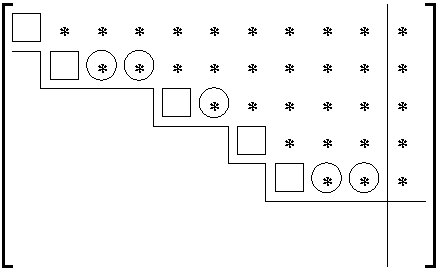
\includegraphics[height=1.25in]{3_hermite1}
\hspace{5mm}
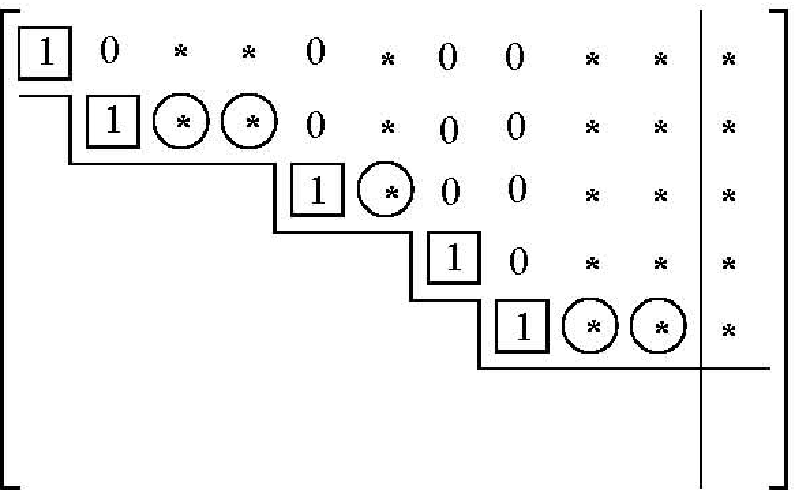
\includegraphics[height=1.25in]{3_hermite1rref}}
\caption{After Gaussian Elimination the augmented matrix will be 
in row echelon form (left). With further work, the augmented matrix can 
be put in reduced row echelon form (right). 
\label{fig_hermite1}}
\end{figure}

If we want to put this example in completely reduced form, we
use elementary row operations to zero out the entries
lying above the boxes too. Then we
multiply each row by a number so that the corner entries (in the boxes)
become $1$. The completely reduced form for the example above 
would look like the diagram in Figure~\ref{fig_hermite1} (right). 
The official name of this form is the {\em reduced row echelon form}.

If the bottom of the matrix has a row that is all zeroes, except for the
augmented entry, then the system of equations has no solutions. This is because
the bottom row stands for an equation of the form $0=\Box$ with $\Box\ne 0$.
A typical example is shown in Figure~\ref{fig_hermite2} (left). 

\begin{figure}
\centerline{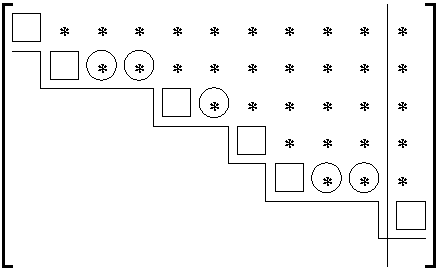
\includegraphics[height=1.5in]{3_hermite2}
\hspace{5mm}
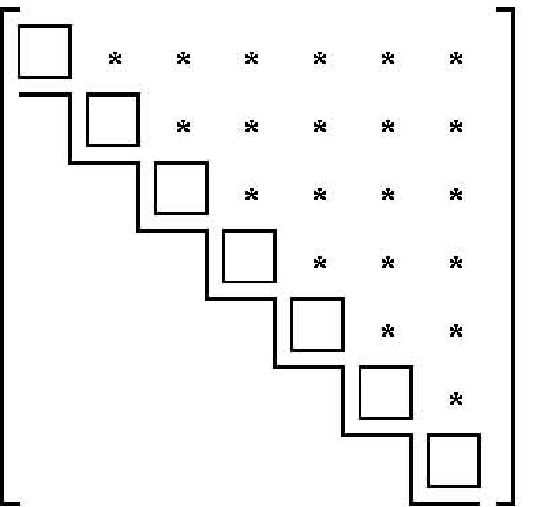
\includegraphics[height=1.5in]{3_hermite3}}
\caption{Augmented matrices after Gaussian Elimination 
with no solutions (left) and with a single solution (right). 
\label{fig_hermite2}}
\end{figure}

If all the steps on the staircase in the non-augmented part of the matrix
have size one, then there are no parameters to introduce, and the solution is
unique. Notice that in this case there are the same number of equations as
variables. A typical example is shown in Figure~\ref{fig_hermite2} (right). 

Finally, we introduce some terminology.
The {\it rank} of a matrix is the number of non-zero rows in the matrix obtained
after reducing it to the upper triangular form described above. In other words
the rank is the number of boxes in the diagrams above. We can now rephrase the
different possibilities in terms of rank. If the rank of the augmented matrix is
greater than the rank of the unaugmented matrix (i.e., the matrix without the
last column) then there are no solutions. If the rank of the matrix is equal
to the number of unknowns then the solution is unique. If the rank $r$ of the matrix
is equal to the rank of the unaugmented matrix, but less than the number $n$ of
unknowns, then there are $n-r$ parameters in the solution.

Ordinary arithmetic errors are a common source of errors when you do row operations
by hand. There is a technique called ``the check column'' that can often catch such errors. It is described in Section~\ref{s:check}. Another easy way to make sure that we have not made any mechanical errors in calculating the solution of a linear system is just to substitute the purported solution
back into the original system and verify that each left hand side really is equal to its corresponding
right hand side.

\subsection{Using MATLAB for row reductions}

MATLAB has a built in command
called {\tt rref} that reduces a matrix to reduced row echelon form.
Let us  try it on the example in the previous section. First we define
the initial matrix {\tt A}. Remember that the last column of this matrix is
the augmented part.
\begin{verbatim} 
A = [1 2 -2 -7 -29; 1 2 -1 -5 -18; 0 3 0 -3 -6; -1 4 1 1 14]
\end{verbatim}
To find the reduced row echelon form, simply type
\begin{verbatim}
>> rref(A)
ans = 
1 0 0 0 1
0 1 0 0 2
0 0 1 0 3
0 0 0 1 4
\end{verbatim}
Notice that this MATLAB command did the work of Examples~\ref{ex_gebs} 
and~\ref{ex_rref}. The solution to the system can be read off the result
of the {\tt rref} command above. 

It is important to realize that floating point rounding errors as discussed in 
Section~\ref{sec:floating} can lead to errors in solutions to linear systems computed 
by MATLAB and other computational tools. At worst, these errors will lead to MATLAB 
finding ``solutions'' to problems that do not have exact solutions. In these cases, 
solutions will often have very large values and often MATLAB will give a warning 
about the problem being ``ill-conditioned".   

\subsection{Problems}

\begin{problem}
\label{op2_2}
Show that the lower triangular system of equations represented by
\[
\left[\matrix{
1&  0&  0\cr
1&  -1& 0\cr
2&  1&  -8\cr
}\right|\left .\matrix{
3\cr
3\cr
-4\cr
}\right]
\]
is also easily solved, by easily solving it! It's just a matter of convention
whether we aim for upper triangular or lower triangular systems in the
elimination procedure.
\end{problem}

\begin{problem}
\label{op2_3}
The following equations have already
been put in upper triangular form. In each case there are infinitely
many solutions, depending on one or more parameters.  Write down the
general expression for the solution in terms of parameters.
\[
\left[
\begin{array}{cccc}
1&2&1&2 \\
0&0&1&1 \\
0&0&0&1 \\
0&0&0&0 \\
\end{array} \right| \left.
\begin{array}{c}
1 \\ 4 \\ 2 \\ 0
\end{array}
\right]
\]

\[
\left[
\begin{array}{cccc}
1&2&1&2 \\
0&0&1&1 \\
0&0&0&0 \\
0&0&0&0 
\end{array} \right| \left.
\begin{array}{c}
1 \\ 4 \\ 0 \\ 0
\end{array}
\right]
\]

\[
\left[\matrix{
1&2&1&2\cr
0&0&1&1\cr
}\right.\left|\matrix{
1\cr 4\cr
}\right]
\]
\end{problem}

\begin{problem}
\label{2009_a4_3}
Consider the system of equations represented by the augmented matrix
\[
\left[
\begin{array}{c c c c | c}
1 & 2 &2 & 2 & 1\\
1 & 3& -1&3 & -1\\
1&0 &1 &1 & 5 \\
0& 3 & -2 & 2 & -6
\end{array}
\right]
\]
Show that this set of equations has infinitely many solutions and find a general parametric representation of the solutions.
\end{problem}

\begin{problem}
\label{2009_a4_1}
Consider the system of equations represented by the augmented matrix
\[
\left[
\begin{array}{c c c c | c}
1 & 2 &2 & -7 & 20\\
3 & 6& -3&-5 &-15\\
0&6 &0 &-6 & -10 \\
2& -8 & -2 & -2 & 30
\end{array}
\right]
\]
Put this matrix in upper triangular form and find the solution of the linear system of equations. You can leave your answers in fractions but show the operations you perform in full detail. 
\end{problem}

\begin{problem}
\label{op2_4}
Solve the following system of equations.
\[
\matrix{
x_1 &-& 2x_2 &+& 3x_3 &=& 2\cr
2x_1 &-& 3x_2 &+& 2x_3 &=& 2\cr
3x_1 &+& 2x_2 &-& 4x_3 &=& 9\cr
}
\]
\end{problem}

\begin{problem}
\label{op2_5}
Solve the following system of equations.
\[
\matrix{
2x_1 &+& x_2 &-& 1x_3 &=& 6\cr
x_1 &-& 2x_2 &-& 2x_3 &=& 1\cr
-x_1 &+& 12x_2 &+& 8x_3 &=& 7\cr
}
\]
\end{problem}

\begin{problem}
\label{op2_6}
Solve the following system of equations.
\[
\matrix{
x_1 &+& 2x_2 &+& 4x_3 &=& 1\cr
x_1 &+& x_2 &+& 3x_3 &=& 2\cr
2x_1 &+& 5x_2 &+& 9x_3 &=& 1\cr
}
\]
\end{problem}

\begin{problem}
\label{op2_7}
Solve the following system of equations.
\[
\matrix{
x_1 &+& 2x_2 &+& 4x_3 &=& 1\cr
x_1 &+& x_2 &+& 3x_3 &=& 2\cr
2x_1 &+& 5x_2 &+& 9x_3 &=& 3\cr
}
\]
\end{problem}

\begin{problem}
\label{op2_8}
Solve the following system of equations.
\[
\matrix{
3x_1 &+& x_2 &-& x_3 &+& 2x_4 &=& 7\cr
2x_1 &-& 2x_2 &+& 5x_3 &-& 7x_4&=& 1\cr
-4x_1 &-& 4x_2 &+& 7x_3 &-& 11x_4&=& -13\cr
}
\]
\end{problem}

\begin{problem} 
\label{op2_9}
For what values of $a$, $b$, $c$, $d$, $\alpha$ and $\beta$ does
the system of equations
\[
\matrix{
ax_1 &+& bx_2 &=& \alpha\cr
cx_1 &+& dx_2 &=& \beta\cr
}
\]
have a unique solution?
\end{problem}

\begin{problem}
\label{2009_a4_2}
Consider the system of equations represented by the augmented matrix
\[
\left[
\begin{array}{c c c | c}
1 & 2 & 0 & 7\\
4 & 8 & 6 & 10\\
-4 & -8 & 10 & 81
\end{array}
\right]
\]
How many solutions does this linear system of equations have?
\end{problem}

\begin{problem}
\label{matlab_2009_a4_2}
(Matlab) Consider the following system of equations
\[
\matrix{
x_1 &+& 2x_2 &+& 4x_3 &=& 7\cr
4x_1 &+& x_2 &+& 3x_3 &=& 2\cr
0 &+& 5x_2 &+& 9x_3 &=& a\cr
}
\]
\end{problem}
Write a script in Matlab that generates the augmented matrix and solves the system with the {\tt rref} command for various values of $a$. Specifically, how does the solution of {\tt $x_1$} vary when you range $a$ from 1 to 10 (equally spaced)?

\section{Homogeneous Equations} 

If the coefficients on the right sides of a system of equations are all zero,
the system is said to be {\it homogeneous}. In other words, a homogeneous system
is a system of equations of the form
\[
\matrix{
b_{1,1}x_1      &+&b_{1,2}x_2   &+\cdots        &+&b_{1,n}x_n   &= &0\cr
b_{2,1}x_1      &+&b_{2,2}x_2   &+\cdots        &+&b_{2,n}x_n   &= &0\cr
\vdots          &\vdots&                &       &&\vdots                &&\vdots
\cr
b_{m,1}x_1      &+&b_{m,2}x_2   &+\cdots        &+&b_{m,n}x_n   &= &0\cr
}
\]
Given a system of equations, the {\it associated homogeneous system} is the
homogeneous system of equations you get by setting all the right sides to zero.

Geometrically, homogeneous systems describe points, lines and planes that pass through the origin. In fact $\xx=\zv$, i.e.,
$x_1=0, x_2=0, \ldots, x_n=0$ is always a solution to a homogeneous system of equations.

When are there {\em{other (nonzero)}} solutions to the above homogeneous system? We have $n$ unknowns and $m$ equations.
When we perform the Gaussian reduction, the right-hand sides of the equations will stay zero
so the augmented matrix will generally have the form
\[
\left[\matrix{ 1&  *&  *& *& \cdots&\cdots&\cdots&*\cr  0&  1&  *& *&  \cdots&\cdots&\cdots& *\cr 0&  0&  0& 1&  *
&\cdots&\cdots& *\cr  \cdots&\cdots&\cdots&\cdots&\cdots&\cdots&\cdots&\cdots\cr  0&  0&  0& \cdots&0& 1& *&  * \cr  0& 0&
0& \cdots& \cdots& \cdots &1&*\cr  0&  0&  0& \cdots&0& 0& 0&  1 \cr
\cdots&\cdots&\cdots&\cdots&\cdots&\cdots&\cdots&\cdots\cr 0&  0&  0& \cdots&0& 0& 0& 0\cr
  }\right|\left .\matrix{ 0\cr0\cr0\cr \cdots \cr0\cr0\cr 0\cr\cdots\cr 0\cr }\right].
\]
The last several lines may be identically zero. In the last section we saw
that there are solutions depending on parameters if the number of variables
is greater than the rank of the matrix. Thus,
if $n$ (the number of unknowns) is bigger
than the number of non-zero lines in the above row-reduced matrix, 
then there exists a non-zero solution. Otherwise only a
trivial solution $x_1=0, x_2=0, \ldots, x_n=0$ is present. 
We illustrate the idea with some examples below.

\begin{example}
Consider a homogeneous system
\[
\matrix{ 3x_1      &+& 6 x_2   &+&x_3   &= &0\cr 6x_1      &+& 2 x_2   &+&2 x_3   &= &0\cr x_1      &+&  x_2   &+&3 x_3 &=
&0\cr}
\]
{\rm The augmented matrix can be reduced by row operations to the form (check!)
\[
\left[\matrix{ 1&  0&  0\cr 0&  1&  0\cr 0&  0&  1\cr }\right|\left .\matrix{ 0\cr 0\cr 0\cr }\right],
\]
which implies $x_1=x_2=x_3=0$. And, in agreement with our above statement, the number of variables (3) is not more than the
number of non-zero rows (also 3).}
\end{example}

\begin{example}
Consider another homogeneous system:
\[
\matrix{ -x_1      &+& 2 x_2   &+&4x_3   &= &0\cr 2x_1      &-& 4 x_2   &-&8 x_3   &= &0\cr x_1      &-&  x_2   &+&3 x_3 &=
&0\cr}.
\]
{\rm Its augmented matrix is 
\[
\left[\matrix{ -1&  2&  4\cr 2&  -4&  -8\cr 1&  -1&  3\cr }\right|\left .\matrix{ 0\cr 0\cr 0\cr }\right] ~\rightarrow~
\left[\matrix{ -1& 2& 4\cr 0&  0&  0\cr 0&  1&  7\cr }\right|\left .\matrix{ 0\cr 0\cr 0\cr }\right]~\rightarrow~
\left[\matrix{ 1& 0& 10\cr 0&  1&  7\cr 0&  0&  0\cr }\right|\left .\matrix{ 0\cr 0\cr 0\cr }\right],
\]
and the number of nonzero rows is 2, which is less than the number of unknowns, 3. Hence by the above statement there must
be a nonzero solution. We find $x_1=-10x_3$, $x_2=-7x_3$, with no 
requirement on $x_3$. Hence $x_3$ is any number $t$, and we
obtain infinitely many nonzero solutions
\[
x_1=-10t, \mbox{\ \ } x_2=-7t, \mbox{\ \ } x_3=t,~~~~t\in (-\infty,\infty),
\]
one for each value of t.}
\end{example}

In a similar manner, if for some homogeneous system with 4 variables the augmented matrix has only 2 nonzero rows, then the
general solution has 4-2=2 free (undefined) variables on which the other two depend.

\subsection{Properties of solutions of homogeneous systems.}

\begin{enumerate}
\item A homogeneous system has either one zero-solution $(x_1=...=x_n=0)$ or infinitely-many solutions that depend on
parameters.
\item If $(x_1,...,x_n)$ and $(y_1,...,y_n)$ are solutions to a given homogeneous system, $(x_1+y_1,...,x_n+y_n)$ is
also a solution. (Solutions are additive.)
\item If $(x_1,...,x_n)$ is a solution to a given homogeneous system, $(ax_1,...,ax_n)$ is also a solution, for any
number $a$. (Solutions are scalable.)
\end{enumerate}

The first statement follows from our previous discussion; the other two are easy to verify, using the initial homogeneous
system.

\subsection{Connection of solutions to homogeneous and inhomogeneous systems.}

The importance of homogeneous equations comes from the following fact. If $\xx=[x_1,x_2,\ldots,x_n]$ and
$\yy=[y_1,y_2,\ldots,y_n]$ are two solutions to a (not necessarily homogeneous) system of equations,
\[
\matrix{
b_{1,1}x_1      &+&b_{1,2}x_2   &+\cdots        &+&b_{1,n}x_n   &= &c_1\cr
b_{2,1}x_1      &+&b_{2,2}x_2   &+\cdots        &+&b_{2,n}x_n   &= &c_2\cr
\vdots          &\vdots&                &       &&\vdots                &&\vdots
\cr
b_{m,1}x_1      &+&b_{m,2}x_2   &+\cdots        &+&b_{m,n}x_n   &= &c_m\cr
}
\]
then the difference
$\xx-\yy=[x_1-y_1,x_2-y_2,\ldots,x_n-y_n]$ solves the associated homogeneous
system. This is a simple calculation
\[
\matrix{
b_{1,1}(x_1-y_1)      &+&b_{1,2}(x_2-y_2)   &+\cdots        &+&b_{1,n}(x_n-y_n)
 &= &(c_1-c_1) &= &0\cr
b_{2,1}(x_1-y_1)      &+&b_{2,2}(x_2-y_2)   &+\cdots        &+&b_{2,n}(x_n-y_n)
 &= &(c_2-c_2) &= &0\cr
\vdots          &\vdots&                &       &&\vdots                &&\vdots
\cr
b_{m,1}(x_1-y_1)      &+&b_{m,2}(x_2-y_2)   &+\cdots        &+&b_{m,n}(x_n-y_n)
 &= &(c_m-c_m) &= &0\cr
}
\]
To see the implications of this let us  suppose that $\xx=\qq$ is any particular
solution to a (non-homogeneous) system of equations. Then if $\yy$ is any other
solution $\yy-\xx=\zz$ is a solution of the corresponding homogenous system.
So $\yy=\qq+\zz$. In other words any solution can be written as $\qq +$ some
solution of the corresponding homogenous system. Going the other way, if
$\zz$ is any solution of the corresponding homogenous system, then $\qq+\zz$
solves the original system. This can be seen by plugging $\qq+\zz$ into the
equation. So the structure of the set of solutions is
\[
\xx = \qq + (\mbox{{\ \bf solution to homogeneous system}})
\]
As you run through all solutions to the homogenous system on the right,
$\xx$ runs through all solutions of the original system. Notice that it doesn't
matter which $\qq$ you choose as the starting point. This is completely analogous
to the parametric form for a line, where the base point can be any
point on the line.

If we have applied the process of
Gaussian elimination to the original system, and concluded that
the general solution has  parameters, we will end up with a general solution of
the form
\[
\qq + s_1\aa_1+\cdots +s_n\aa_n.
\]
Notice that $\qq$ is a particular solution (corresponding to all parameters
equal to zero) and $s_1\aa_1+\cdots +s_n\aa_n$ is the general solution to the
corresponding homogeneous system.

These considerations have practical importance if you have to solve a bunch of
systems, all with the same coefficients on the left side, but with different
coefficients on the right. In this situation, you could first find the general
solution to the corresponding homogeneous system of equations. Then to find the
general solution to one of the systems, you would only need to find a single
particular solution, and then add the general solution to the homogeneous system
to obtain all solutions. The only trouble with this is that it might not really
be any easier to find a single particular solution than it is to find all
solutions.

\begin{example}
\label{op2_10}
Find the general solution of the system of equations
\[
\left[\matrix{
1&1&0&0\cr
-1&-1&1&2\cr
3&3&-1&-2\cr
}\right . \left |\matrix{
1\cr 1\cr 1\cr
}\right]
\]
In the form $\xx=\qq+s_1\aa_1+s_2\aa_2$. Verify that $\aa_1$ and $\aa_2$ solve
the corresponding homogeneous equation.
{\rm The matrix 
\[
\left[
\begin{array}{cccc}
1&1&0&0 \\
-1&-1&1&2 \\
3&3&-1&-2
\end{array} \right| \left.
\begin{array}{c}
1 \\ 1 \\ 1
\end{array}
\right]
\]
reduces to
\[
\left[
\begin{array}{cccc}
1&1&0&0 \\
0&0&1&2 \\
0&0&0&0
\end{array} \right| \left.
\begin{array}{c}
1 \\ 2 \\ 0
\end{array}
\right]
\]
so the solutions are
$x_1=1-s_1$, $x_2=s_1$, $x_3=2-2s_2$, $x_4=s_2$. This can be written
\[
\xx = \left[\matrix{1\cr 0\cr 2\cr 0\cr}\right] + s_1\left[\matrix{-1\cr 1\cr 0\cr 0\cr}\right]
+s_2\left[\matrix{0\cr 0\cr -2\cr 1\cr}\right] 
\]
It's easy to check that $\aa_1=[-1,1,0,0]$ and $\aa_2=[0,0,-2,1]$ solve the 
corresponding homogeneous system.}
\end{example}

\subsection{Problems} 

\begin{problem}
\label{2009_a4_4}
Find the general solution of the system of equations
\[
\left[
\begin{array}{c c c c | c}
1 & 0 &1 & 0 & 10\\
-1 & 1& 1&1 & 4\\
0&1 &2 &1 & 14
\end{array}
\right]
\]
In the form $ {\bf x} = {\bf q} + s_1 {\bf a}_1+ s_2 {\bf a}_2$, where ${\bf a_1}$ and ${\bf a}_2$ solve the corresponding homogeneous system of equations. 
\end{problem}

\begin{problem}
\label{op2_11}
Consider the system of equations
\[
\left[\matrix{
1&1&0&0\cr
-1&-1&1&2\cr
3&3&-1&-2\cr
}\right . \left |\matrix{
4\cr -1\cr 9\cr
}\right]
\]
Verify that $[4,0,3,0]$ is a solution and write down the general solution.
\end{problem}

\begin{problem}
\label{2009_a4_5}
Consider the system of equations given by the augmented matrix
\[
\left[
\begin{array}{c c c  | c}
1 & -3 &4 & 6 \\
1 & 9& -10&10 \\
0&6 &-7 &2
\end{array}
\right]
\]
Put this matrix in reduced row echelon form and comment on the number of solutions of this system of equations. 
\end{problem}

\section{Geometric Applications}
\label{s:geom}

Now we will apply Gaussian elimination to some of the geometry problems
we studied in the first part of this course. 

Let us start with the question of linear independence. Recall that a collection
of vectors $\xx_1, \xx_2, \ldots, \xx_n$ is called linearly dependent if
we can find some non-zero coefficients $c_1, c_2, \ldots, c_n$ such that
\[
c_1\xx_1 + c_2\xx_2 + \cdots + c_n\xx_n = \zv
\]
This is actually a homogeneous system of linear equations for the numbers
$c_1, \ldots, c_n$. If $c_1=c_2=\cdots =c_n=0$ is the only solution, then
the vectors are linearly independent. Otherwise, they are linearly dependent.
To decide, we must set up the matrix for the system of equations and
perform a row reduction to decide if there is a unique solution or not.
In setting up the equations, it is convenient to treat the $\xx_i$'s as column
vectors.

\begin{example}
\label{ex_linind}
Decide if 
\[
\xx_1=\left[\matrix{1\cr 2\cr 0\cr}\right] \quad
\xx_2=\left[\matrix{1\cr 1\cr 1\cr}\right] \quad
\xx_3=\left[\matrix{1\cr 2\cr 1\cr}\right]
\]
are linearly independent. 
{\rm The equation $c1\xx_1+c_2\xx_2+c_3\xx_3=\zv$
can be written
\[
\matrix{
c_1 &+ c_2 &+ c_3 &= 0\cr
2c_1 &+c_2 &+ 2c_3 &= 0\cr
0c_1 &+c_2 &+c_3 &= 0\cr
}
\]
The matrix for this system of equations is
\[
\left[\matrix{
1&1&1\cr
2&1&2\cr
0&1&1\cr
}\right]
\]
Since this is a homogeneous system, we don't have to write
the augmented part of the matrix. Performing a row reduction
yields 
\[
\left[\matrix{
1&1&1\cr
0&1&0\cr
0&0&1\cr
}\right]
\]
Since the number of non-zero rows is the same as the number of variables
(three) there are no non-zero solutions. Therefore the vectors are
linearly independent.}
\end{example}

The row reduction in Example~\ref{ex_linind} 
also shows that any vector $\yy$ in $\RR^3$
can be written as a linear combination of $\xx_1$, $\xx_2$ and $\xx_3$.
Writing $\yy$ as a linear combination of $\xx_1$, $\xx_2$ and $\xx_3$
means finding coefficients $c_1$, $c_2$ and $c_3$ such that
$c1\xx_1+c_2\xx_2+c_3\xx_3=\yy$. This is a (non-homogeneous)
system of linear equations with augmented matrix
\[
\left[\matrix{
1&1&1\cr
2&1&2\cr
0&1&1\cr}\right|\left.\matrix{
y_1\cr y_2\cr y_3\cr
}\right]
\]
Using the same Gaussian elimination steps as above, this matrix 
reduces to
\[
\left[\matrix{
1&1&1\cr
0&1&0\cr
0&0&1\cr}\right|\left.\matrix{
*\cr*\cr*\cr
}\right]
\]
where the $*$'s are some numbers. This system has a (unique)
solution.

\begin{example}
Here is another geometric example. Do the planes whose
equations are given by $x_1+x_2+x_3=1$, $2x_1+x_2+2x_1=1$ and
$x_2=1$ intersect in a single point? 
{\rm To answer this, we note
that the intersection of the three planes is given by the set
of points that satisfy all three equations. In other words they
satisfy the system of equations whose augmented matrix is
\[
\left[\matrix{
1 & 1 & 1\cr
2 & 1 & 2\cr
0 & 1 & 0\cr
}\right|\left.\matrix{
1\cr 1\cr 1\cr
}\right]
\]
A row reduction yields
\[
\left[\matrix{
1 & 1 & 1\cr
0 & -1 & 0\cr
0 & 0 & 0\cr
}\right|\left.\matrix{
1\cr -1\cr 0\cr
}\right]
\]
Thus solutions are given by
\[
\left[\matrix{0\cr 1\cr 0\cr}\right] + s \left[\matrix{1\cr 0\cr -1\cr}\right]
\]
This is the parametric equation of a line. Thus the three planes intersect
in a line, not a point.}
\end{example}

\subsection{Problems}

\begin{problem}
\label{op2_12}
Are the following vectors linearly dependent or
independent?
\[
\xx_1=\left[\matrix{1\cr 2\cr 0\cr 2\cr}\right] \quad
\xx_2=\left[\matrix{1\cr 1\cr -1\cr 1\cr}\right] \quad
\xx_3=\left[\matrix{1\cr 0\cr 1\cr 0\cr}\right]
\]
Can every vector in $\RR^4$ be written as a linear combination of
these vectors? How about the vector the  
\[
\yy_1=\left[\matrix{2\cr 4\cr -3\cr 4\cr}\right]? 
\]
\end{problem}

\begin{problem}
\label{2009_a5_1}
Consider the following vectors ${\bf a}_1$, ${\bf a}_2$ and ${\bf a}_3$ such that:
\[{\bf a}_1 = \left[\begin{array}{c}
1\\
2
\end{array}\right]\hspace{4mm}{\bf a}_2 = \left[\begin{array}{c}
3\\
1
\end{array}\right]\hspace{4mm}{\bf a}_3 = \left[\begin{array}{c}
-3\\
4
\end{array}\right]\]
Are they linearly independent? Can the vector ${\bf y}=\left[\begin{array}{c} -15\\ 5\end{array}\right]$ be written as a linear combination of ${\bf a}_1$ and ${\bf a}_2$?
\end{problem}

\begin{problem}
\label{2009_a5_2}
Consider the following 4 dimensional vectors $\aa_1$, $\aa_2$, and $\aa_3$ such that
$$
a_1 = \left[\begin{array}{c} 1\\1\\0\\0 \end{array}\right] \qquad
a_2 = \left[\begin{array}{c} 0\\0\\4\\-3 \end{array}\right] \qquad
a_3 = \left[\begin{array}{c} 10\\0\\-5\\0 \end{array}\right]
$$
Are these linearly independent? Can the vector $\boldmath{y}$ below be written as  linear combination of the above three vectors?

\end{problem}

\begin{problem}
\label{matlab_2009_a5_2}
(Matlab) Consider the following 3 vectors $\aa_1$, $\aa_2$, and $\aa_3$:
$$
a_1 = \left[\begin{array}{c} 1\\2\\3 \end{array}\right] \qquad
a_2 = \left[\begin{array}{c} -1\\2\\-1 \end{array}\right] \qquad
a_3 = \left[\begin{array}{c} 4\\1\\-1 \end{array}\right]
$$
The Matlab command
\begin{verbatim}
  plot3([a,0], [b,0], [c,0])
\end{verbatim}
draws a line between $(0,0,0)$ and a point with coordinates $(a,b,c)$. Write a script that draws the three vectors (use the command {\tt hold on} to be able to overlap them). Are the vectors linearly independent?

\end{problem}

\section{Resistor Networks}
\label{sec_res_networks}
\subsection{Elements of Basic Circuits}

Electrical current, often denoted with the variable $I$, is a measure 
of charge flow with MKS units of Amperes or Amps (Coulombs per second, 
where a Coulomb is a measure of electrical charge). The voltage $V$ 
is an electrical potential measured in Volts (Joules per Coulomb). Thus 
$IV$ has the units of power (J/s or Watts). 

A resistor is a simple electrical component that obeys Ohm's law, 
that the current through it is proportional to the voltage drop across it. 
The constant of proportionality is called the resistance $R$ in Ohms
(abbreviated $\Omega$, V/A). The current $I$ through a resistor across 
which there is a voltage drop $V$ satisfies 
\[
V = IR.
\]
The current goes from high to low potential through the resistor. 

The resistor networks considered in these notes are circuits with three 
types of components:
\begin{enumerate}
\item Resistors 
\item Voltage sources 
\item Current sources 
\end{enumerate}
The notation we will use for these elements in circuit schematics 
is shown in Figure~\ref{fig_elements}. Later (in Chapter 5) 
we will see that such a 
network represents a network with additional elements (inductors 
and capacitors) at a given instant in time. At a given time, an inductor 
acts as a current source and a capacitor acts as a voltage source. 
The current through the capacitor at that instant determines the rate 
of change of voltage across it, and the voltage across the inductor 
determines the rate of change of current through it. 

\begin{figure}
\centerline{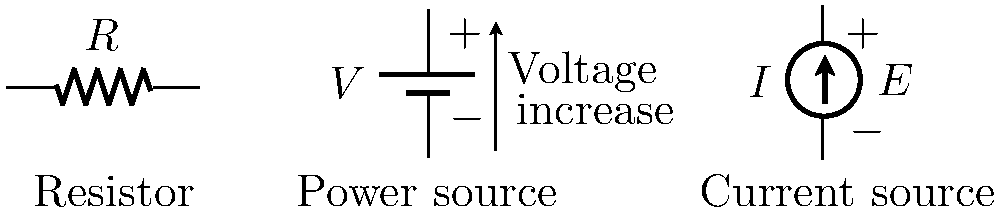
\includegraphics[width=4in]{3_elements}}
\caption{Elements in resistor networks. 
\label{fig_elements}}
\end{figure}

In the network, the resistances of all resistors will be given. The 
voltage across all voltage sources and the currents through all current 
sources will be given. 
There are two basic questions to answer about a resistor network with these
components. 
\begin{description}
\item[basic problem:] Find the currents through each resistor 
and each power source and also the voltage drops across each 
current source. This problem is a {\em linear system} of equations and 
so serves as an example of the mathematical techniques learnt in this 
chapter. 
\item[fundamental problem:] An important sub-problem is to find the 
currents through every power source and the voltage drops across 
each current source. These quantities can be written in terms of the given 
voltages and current sources directly (eliminating the terms involving 
resistor currents). 
Later, solving this problem will tell us how to 
write a differential equation for the currents through inductors and 
the voltages across capacitors. 
\end{description}

There are two fundamental laws governing the behaviour of circuits that 
can be used to set up equations that can be solved to answer the questions 
above. They are Kirchhoff's laws:
\begin{enumerate}
\item The sum of voltage drops around any closed loops in the network 
must be zero. 
\item The sum of currents entering a node must be zero. 
\end{enumerate}

\subsection{Two Simple Examples Made Complicated}

Consider the simple network with one current source and one resistor 
shown in Figure~\ref{fig_simple} (left). Clearly, the current 
through the resistor must be $I$ and the voltage drop across the 
resistor must be $IR$ using Ohms Law (use the signs in the diagram 
for the direction of the drop). 


\begin{example}
\label{Ex:simple1} 
Consider the same example, introducing two nodes into the network 
as shown in Figure~\ref{fig_simple} (right). We now have three unknowns, 
$V_1$, $V_2$ and $I_2$. Find a linear system for these unknowns 
and then solve the system.
{\rm We have made this simple example more complicated 
but we will learn something as we work through it. Note that by specifying 
voltages at nodes (which will determine voltage drops across components)
we will always satisfy Kirchhoff's first law. Let us write down every other 
law that applies to this diagram:
\begin{eqnarray*}
I - I_2 & = & 0 \mbox{,\ \ Kirchhoff's second law at node 2} \\
I_2 - I & = & 0 \mbox{,\ \ Kirchhoff's second law at node 1} \\
V_2 - V_1 & = & I_2 R \mbox{,\ \ Ohm's Law over the resistor} 
\end{eqnarray*}
If you didn't look too closely, you might be happy thinking these 
are three equations for the three unknowns $I_2$, $V_1$ and $V_2$. 
However, rewriting gives 
\begin{eqnarray*}
I_2 & = & I \\
I_2 & = & I \\
V_2 - V_1 - I_2 R & = & 0 
\end{eqnarray*}
In augmented matrix form we can write the system and do Gaussian 
Elimination:
\[
\left[
\begin{array}{ccc}
1 & 0 & 0 \\
1 & 0 & 0 \\
-R & -1 & 1 
\end{array}
\right|
\left.
\begin{array}{ccc}
I \\ I \\ 0 
\end{array}
\right]
\sim 
\left[
\begin{array}{ccc}
1 & 0 & 0 \\
0 & -1 & 1 \\
0 & 0 & 0
\end{array}
\right|
\left.
\begin{array}{ccc}
I \\ -RI \\ 0 
\end{array}
\right]
\]
In the augmented matrix above, the unknowns are ordered $I_2$, $V_1$ 
and then $V_2$. The solutions are $I_2 = I$ (expected), $V_2 = s$ 
and $V_1 = s-RI$ where $s$ is a parameter that can take any value. 
This seems much more complicated that the intuitive solution at the 
beginning of this section. However, the conclusions are the same: 
the current through the resistor is $I$ and the voltage drop across 
the resistor is 
\[
V_2 - V_1 = s-(s-RI) = RI.
\]
The arbitrary constant in the voltage occurs here 
because no {\em reference} voltage has been specified (no point in the 
circuit has been grounded). }
\end{example} 

\begin{figure}
\centerline{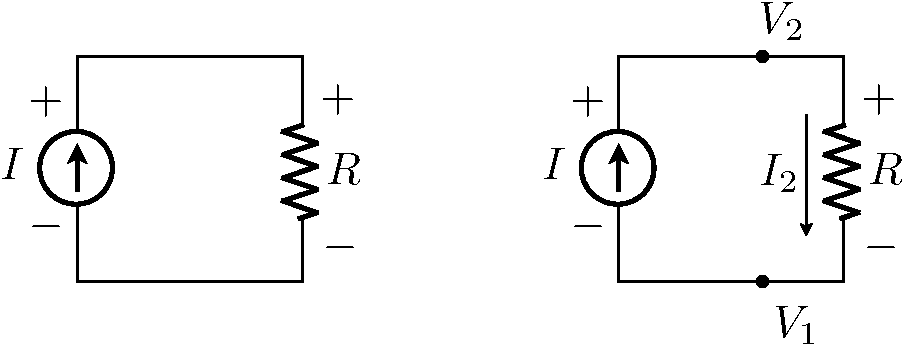
\includegraphics[width=4in]{3_simple}}
%\includegraphics[height=1.5in]{3_simple2}}
\caption{The simple resistor network considered in Example~\ref{Ex:simple1}. 
\label{fig_simple}}
\end{figure}

\begin{example} \label{Ex:simple2} Consider the circuit in Figure~\ref{fig_simple2}. 
Learning from the last example, we have set a reference voltage at the lower 
left corner of the circuit, and then voltage at the upper left corner is 
known. The current $I_1$ is the branch current from the $V_2$ node to the $V_1$ 
node. Form a linear system matching currents and voltages across resistors 
to Ohms Law, and matching branch currents at the two nodes. Solve the linear system.  
{\rm There are 5 unknowns $V_1$, $V_2$, $I_1$, $I_2$ and $I_3$ in the circuit 
as shown in the figure (the augmented matrices below will be written 
with the unknowns in this order). Ohm's law on the four resistors gives the following 
linear equations (in order of small to large resistance) 
\begin{eqnarray*}
12-V_1 & = & I_1 \\
V_1-V_2 & = & 2I_2 \\
V_1-V_2 & = & 3I_3 \\
V_2 & = & 4I_1 
\end{eqnarray*}
and matching the currents at the two nodes gives 
\begin{eqnarray*}
I_1 & = & I_2 + I_3 \\
I_2 + I_3 & = & I_1 
\end{eqnarray*}
This gives six equations in five unknowns! (maybe you already see why this happened 
to us). Writing the six equations above in an augmented matrix gives 
\[
\left[
\begin{array}{ccccc}
-1 & 0 & -1& 0 & 0  \\
1 & -1 & 0 & -2 & 0 \\
1 & -1 & 0 & 0 & -3 \\
0 & 1 & -4 & 0 & 0 \\
0 & 0 & 1 & -1 & -1 \\
0 & 0 & -1 & 1 & 1  
\end{array}
\right|
\left.
\begin{array}{c}
-12 \\ 0 \\ 0\\0\\0\\0
\end{array}
\right]
\sim 
\left[
\begin{array}{ccccc}
1 & 0 & 0 & 0 & 0 \\
0 & 1 & 0 & 0 & 0 \\
0 & 0 & 1 & 0 & 0 \\
0 & 0 & 0 & 1 & 0 \\
0 & 0 & 0 & 0 & 1 \\
0 & 0 & 0 & 0 & 0 
\end{array}
\right|
\left.
\begin{array}{c}
2184/217 \\ 1680/217 \\ 420/217 \\ 252/217 \\ 168/217 \\ 0  
\end{array}
\right]
\]
On the left above is the result of Gaussian elimination to reduced row echelon form. 
The solutions for $V_1$, $V_2$, $I_1$, $I_2$ and $I_3$ can be read off the last column
of the augmented matrix after reduction ($V_1=2184/217$ etc.). Notice that 
the ``extra" equation became the bottom row (all zeros) in the reduced form, which 
indicates that there was redundant information given in the linear system. 
If you go back to the expressions for conservation of current at the two nodes above, 
it is easy to see that these two equations carry the same information. 
}
\end{example}

\begin{figure}
\centerline{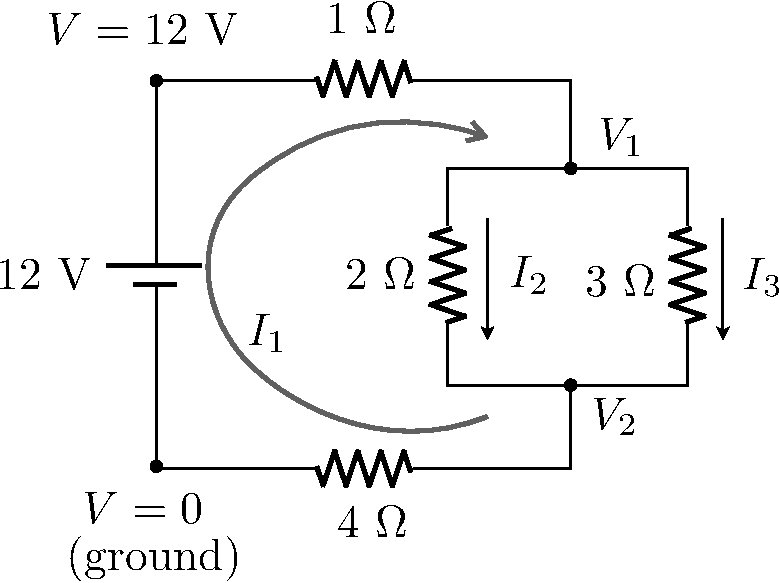
\includegraphics[height=2.5in]{3_resnet2010}}
\caption{The resistor network considered in Example~\ref{Ex:simple2}. 
\label{fig_simple2}}
\end{figure}

As the two previous examples show, one has to be a bit careful picking the unknowns 
and equations in a circuit to get a unique solution without introducing redundant 
equations. There are several ways to do this and when solving small circuits by hand 
the linear system can be made much simpler to solve if you pick the ``right" 
technique. In the next section we will describe the ``loop current" technique which 
always leads to a solvable linear system with no extra (redundant) equations.  

\subsection{Loop Currents}
\label{sec:loop}

We want to be able to see any resistor network and write down equations that 
will solve it uniquely, with no redundant equations like in the previous 
example and no non-uniqueness (like that coming from the 
lack of a reference potential). This can always be done using the 
following variables: loop currents, that is currents in every elementary 
loop of the network, and voltage drops across any current sources. This technique 
is described in more detail below.

Consider a circuit that can be drawn on a piece of paper with no
branches overlapping (a so-called planar network). The branches in the
circuit divide the diagram into smaller areas. The set of branches
around each of these small areas is called an elementary loop. By
assigning a \emph{loop current} to each elementary closed loop of the
circuit, the second of Kirchhoff's Circuit Laws is satisfied
automatically because in a closed loop the current entering any one
point is equal to the current travelling away from that point. Consider
Figure~\ref{labExf} (left). There are three elementary loops and loop
currents $i_1$, $i_2$ and $i_3$ associated with each of them. Loop
currents sum when they overlap in a branch. For example, the current
downwards through the 3 $\Omega$ resistor in Figure~\ref{labExf} is $i_2
- i_3$. Be careful of signs as you sum loop currents. In the example
above, $i_2$ is downwards through the 3 $\Omega$ resistor but $i_3$ is
upwards, hence it appears with a negative sign in our expression.

In a circuit, it is convenient to take loop currents and voltage drops
across current sources as the unknowns.  The first step in solving any
electric network is to identify the number of elementary loops in the
network. If there are $m$ independent loops present, then variables
$i_1,i_2,\ldots,i_m$ must be introduced to represent the loop
currents of each. If there are $n$ current sources, then the variables
$v_1, v_2, \ldots v_n$ must be introduced to represent the voltage
drop across each source. Together there are $n+m$ unknowns.

We can apply Kirchhoff's voltage law to each of the $m$ loops and
obtain $m$ linear equations for the unknowns. The current through each
current source must match the loop currents through it. This gives $n$
more linear equations for a total of $n+m$ linear equations for the
$n+m$ unknowns. 

\begin{example} 
\label{ex_resex2}
Solve the resistor network in Figure~\ref{fig_resex2}. Note that this is the same 
circuit as Example~\ref{Ex:simple2} but here the loop current method 
will be used. 
{\rm The unknowns are the loop currents 
$i_1$ and $i_2$ (there are no current sources). 
Remember that the loop currents add in shared components. For example, 
the current downwards in the 2$\Omega$ resistor is $i_1-i_2$. Using 
loop currents Kirchhoff's second law is always satisfied. The equations 
needed to solve for the loop currents are obtained by summing 
voltage drops around each elementary loop:
\begin{eqnarray*}
i_1 + 2(i_1-i_2) + 4i_1 - 12 & = & 0 
   \mbox{,\ \ voltage drops going around loop 1} \\
3i_2 + 2(i_2 - i_1) & = & 0 
   \mbox{,\ \ voltage drops going around loop 2.} 
\end{eqnarray*}
Collecting terms:
\begin{eqnarray*}
7 i_1 - 2i_2 & = & 12 \\
-2i_1 + 5i_2 & = & 0 
\end{eqnarray*}
which can be solved to give $i_2 = 24/31$ and $i_1 = 420/217$. With 
these values of $i_1$ and $i_2$ the current through each resistor 
and the power source can be determined, solving the problem. }
\end{example}

\begin{figure}
\centerline{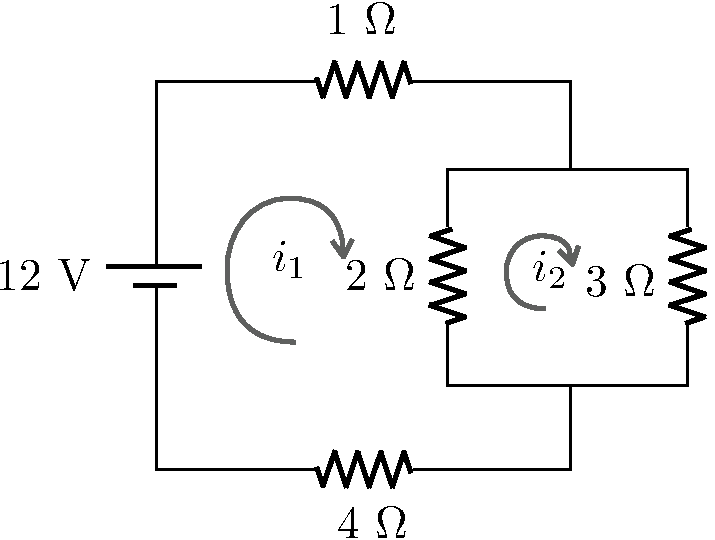
\includegraphics[height=1.5in]{3_resex2}}
\caption{The resistor network for Example~\ref{ex_resex2}
\label{fig_resex2}}
\end{figure}

There are easier ways to solve this {\em particular} small problem (the 
easiest is probably to use combinations of the series and parallel 
resistor laws). However, the loop current rule works for networks 
of arbitrarily large size and leads to systems of equations with a 
relatively small number of unknowns. On tests and exams, it is expected 
that students will be able to apply the idea of loop currents. 

\begin{example} 
\label{labEx} Solve the network shown in Figure~\ref{labExf}
{\rm There are three independent loop
currents which are labelled $i_1$, $i_2$ and $i_3$. There is a single 
current source  of $4A$ with voltage drop $v$ across it (minus to plus in the
direction of the current). There are also two $10V$ voltage sources.
Remember that the
current in an electrical branch shared by two loop currents is equal
to the (signed) sum of the two loops currents, \emph{i.e.} the current
moving to the left through the $5\Omega$ resistor of Figure \ref{labExf} is $i_1-i_
3$ and
thus the voltage drop is $5(i_1-i_3)$. Be careful also of the sign of
voltage drops. Moving around loop 1 in the circuit in Figure~\ref{labExf}
clockwise, when the current source is crossed, there a voltage
increase of $v$, so this would be a voltage {\em drop} of $-v$ in the
expression for Kirchhoff's second law for this loop written below.
We sum the voltage drops around loop 1 beginning at the current source
and moving clockwise (the same direction as $i_1$) to obtain
\[
-v + 2 i_1 + 5(i_1-i_3) + 2(i_1-i_2) = 0
\]
which can be simplified to 
\[
9i_1 -2 i_2 -5 i_3 -v = 0 
\]
The equations for the voltage drops around loops 2 and 3 are derived
similarly 
\[
\begin{array}{ccccccc}
-2i_1&+&5i_2&-& 3i_3 &=& -10 \\
-5i_1&-&3i_2&+& 8i_3 &=& \phantom{-}10
\end{array} 
\]
The final linear equation comes from matching the loop currents to the
current source:
\[
i_1 = 4
\]
The four linear equations above can be solved for the four unknowns $i_1, i_2, i_3, v$. 
The solution can be found using MATLAB (the details are in the computer lab \#4 
guide):
\[
\begin{array}{lcc}
i_1 &=& 4 {\rm A}\\
i_2 &\approx & 2.3871 {\rm A}\\
i_3 &\approx & 4.6452 {\rm A}\\
v & = & 8 {\rm V} 
\end{array}
\]
Now that the loop currents are determined, the branch currents can be
written down. For example the current over the $5\Omega$ resistor to
the right is 
$i_3-i_1 = 0.6452A$. The right hand panel of Figure \ref{labExf} displays
all six branch currents.}
\end{example}

\begin{figure}[htbp]
\centerline{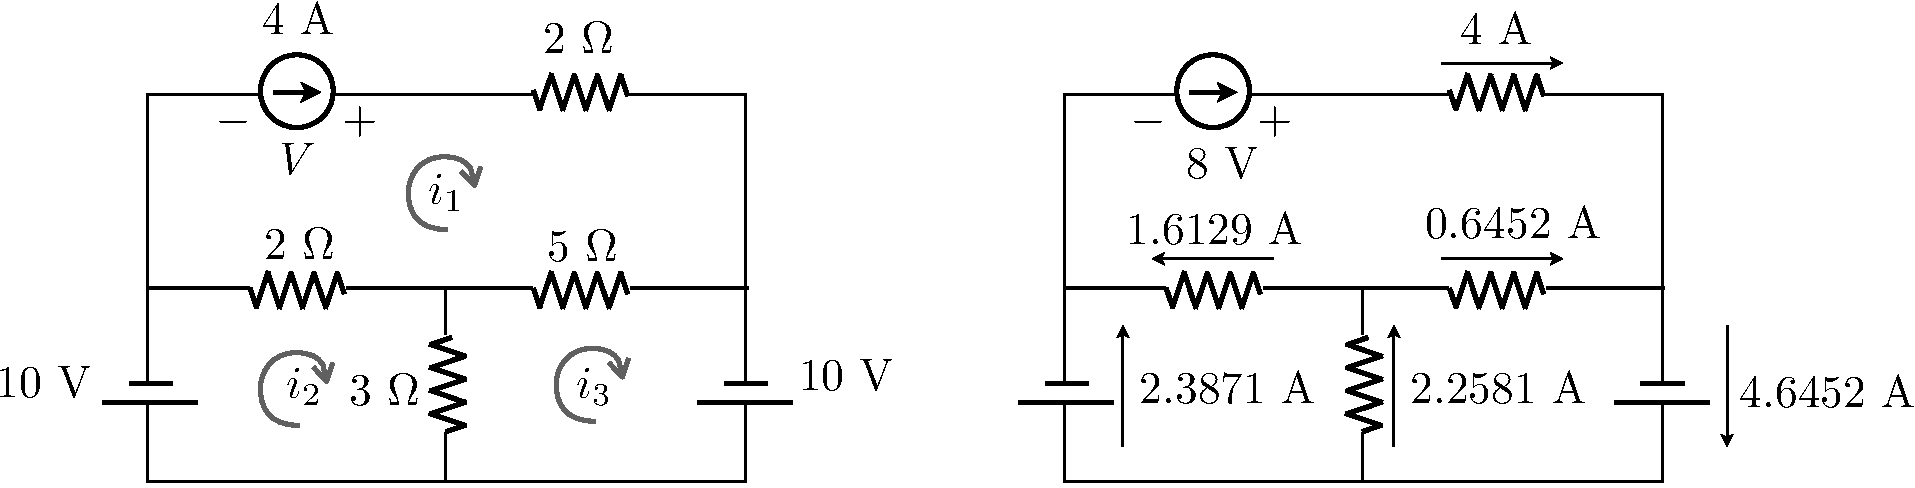
\includegraphics[width=5in]{3_lab4}}
\caption{\label{labExf} The left panel displays the schematic
circuit from Example~\ref{labEx} with two $10V$ voltage sources, 
four resistors and a current
source of $4A$. The loop currents $i_1$, $i_2$ $i_3$ represent the
current in each of the independent closed loops. The right panel is
the solution to the electric network on the left panel with branch
currents shown.}
\end{figure}

\begin{example} 
\label{ex_resex3}
Solve the resistor network in Figure~\ref{fig_resex3}. In this case, solve 
both the basic problem when $V=9$ and $I=1$, and then the fundamental problem
for arbitrary $V$ and $I$. 
{\rm The unknowns for the problem are $i_1$, $i_2$, $i_3$ and $E$. One 
equation in the system of unknowns comes from the fact that the loop 
current variables must match the current source:
\[
i_3= -I.
\]
Note that this equation is so simple we will no longer consider $i_3$ 
as a variable but replace $i_3$ by the known value $-I$ in the 
equations below. 
Voltage drops across the three loops give:
\begin{eqnarray*}
i_1 + 2(i_1-i_2) + 5i_1 - V & = & 0 \\
3(i_2 - i_3) + 2(i_2 - i_1) & = & 0 \\
5 i_3 + E + 3(i_3-i_2) & = & 0 
\end{eqnarray*}
Since $I$ and $V$ and $i_3$ (by the discussion above) are known 
quantities, we move them to the right hand side of the linear 
equations for $i_1$, $i_2$ and $E$ which are written below 
\begin{eqnarray}
\nonumber
8i_1 - 2i_2 & = & V \\
\label{eq_res4}
-2i_1 + 5i_2 & = & -3I \\
\nonumber 
-3i_2 + E & = & 8I.
\end{eqnarray}
With $V=9$ and $I=1$ this is solved using Gaussian Elimination to give 
the solution $E=7 \frac{1}{2}$, $i_2 = -1/6$ and $i_1= 13/12$. Note that the 
negative value for $i_2$ means that this loop current physically goes in the 
opposite direction to that in the Figure. For the 
fundamental problem, we consider (\ref{eq_res4}) for arbitrary values 
of $V$ and $I$. We write the system as an augmented matrix and do 
Gaussian Elimination with symbolic terms in the right hand sides:
\[
\left[
\begin{array}{ccc}
8 & -2 & 0 \\
-2 & 5 & 0 \\
0 & -3 & 1 
\end{array}
\right|
\left.
\begin{array}{c}
V \\ -3I \\ 8I 
\end{array}
\right] 
\sim 
\left[
\begin{array}{ccc}
1 & -1/4 & 0 \\
0 & 1 & 0 \\
0 & 0 & 1 
\end{array}
\right|
\left.
\begin{array}{c}
V/8 \\ -2/3I +V/18 \\ 6I + V/6
\end{array}
\right] 
\]
so $E=6I + V/6$ (the voltage across the current source in terms of the 
given voltage and currents of sources) and (after some algebra) 
$i_1 = \frac{10}{72} V - \frac{1}{6} I$ (the current through the
power source). An alternate approach to solving the fundamental 
problem is given in next section.}
\end{example} 

\begin{figure}
\centerline{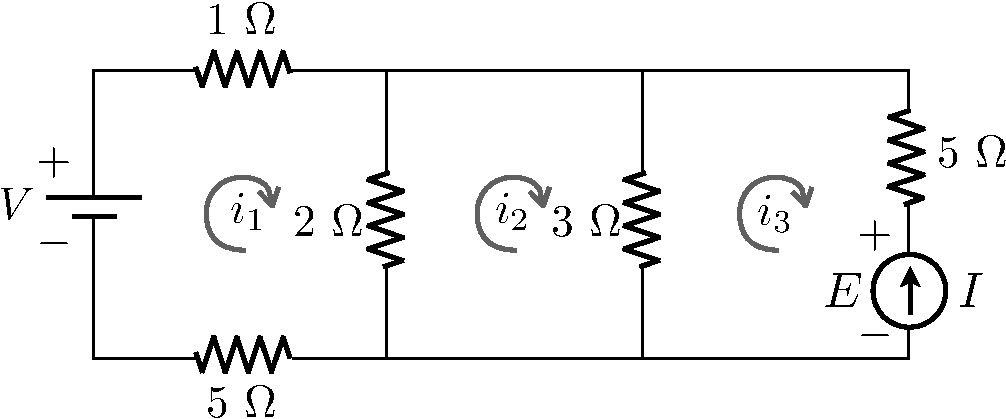
\includegraphics[width=4in]{3_resex3}}
\caption{The resistor network for Example~\ref{ex_resex3}
\label{fig_resex3}}
\end{figure}

\subsection{Alternate Presentation of Resistor Networks}
\label{sub_alternate}

Linear systems from resistor networks was presented in a previous 
version of the notes in a different way. That previous presentation 
is reproduced here beginning in the next paragraph. This alternate 
explanation may be helpful to some students. 

\begin{figure}
\centerline{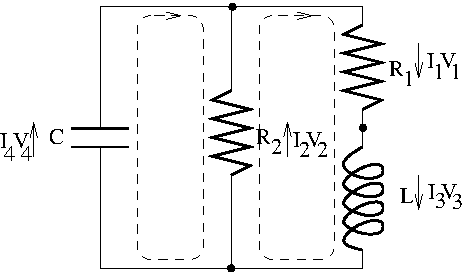
\includegraphics[height=1.5in]{3_circuit}}
\caption{A resistor network. 
\label{fig_circuit}}
\end{figure}

Consider the circuit shown in Figure~\ref{fig_circuit}. 
We won't be able to solve this circuit until we a studied differential equations
in the last part of this course. However we can make some progress
using what we know already.

There are three types of components: 
resistors, inductors (coils) and capacitors.
Associated with each component is the current $I$ flowing through that
component, and the voltage drop $V$ across that component. If there are $n$
different components in a circuit, then there are $2n$ variables (currents and
voltages) to determine. In the circuit above there are $8$.

Of course, these variables are not all independent. They satisfy two types of
linear relations: algebraic and differential. We won't touch the differential
relations for now, but we can consider the algebraic relations.

The first algebraic relation relates the current and voltage drop across a
resistor. If $R$ is the resistance and $I$ and $V$ are the current and voltage
drop respectively, then $V=IR$. In our example, this gives two equations
\begin{eqnarray*}
V_1&=&I_1R_1 \\
V_2&=&I_2R_2 \\
\end{eqnarray*}

The other two algebraic relations are Kirchhoff's laws. The first of these states
that the total voltage drop across any loop in the circuit is zero. For the two
loops in the example circuit, this gives the equations
\begin{eqnarray*}
V_4-V_2&=&0 \\
V_1+V_3+V_2&=& 0
\end{eqnarray*}
Notice we have to take the direction of the arrows into account. The second
Kirchhoff law states that current cannot accumulate at a node. At each node,
the current flowing in must equal the current flowing out. In the example
circuit there are three nodes, giving the equations.
\begin{eqnarray*}
I_4+I_2-I_1&=&0 \\
I_1-I_3&=&0 \\
I_3-I_2-I_4&=&0
\end{eqnarray*}

We now want to pick a few
of the variables, and solve for all the rest in terms of these. In a small
circuit like the example, this can be done ``by hand.''  For example, its pretty
obvious that $I_1=I_3$ and $V_2=V_4$ so one could eliminate two variables right off the
bat.
However, it is also useful
to have a systematic way of doing it, that will work for any circuit (but probably
will require a computer for anything but the simplest circuit).

As a rule of thumb, you can pick the voltages across the capacitor and the
currents across the inductors as basic variables and solve for the rest in
terms of these. In other words, we want $I_3$ and $V_4$ to be {\it parameters}
when we solve the system of equations. To accomplish this we will choose the
order of the variables with $I_3$ and $V_4$ at the end of the list. With this
in mind we choose the order $I_1,I_2,I_4,V_1,V_2,V_3,I_3,V_4$. Then the
equations become
\[
\matrix{
R_1I_1  &   &   &-V_1   &   &   &   &   &=0\cr
    &R_2I_2 &   &   &-V_2   &   &   &   &=0\cr
    &   &   &   &-V_2   &   &   &+V_4   &=0\cr
    &   &   &V_1    &+V_2   &+V_3   &   &   &=0\cr
-I_1    &+I_2   &+I_4   &   &   &   &   &   &=0\cr
I_1 &   &   &   &   &   &-I_3   &   &=0\cr
    &-I_2   &-I_4   &   &   &   &+I_3   &   &=0\cr
}
\]
The matrix for this system is (since it is a homogeneous system of equations,
we don't have to bother writing the augmented part)
\[
\left[\matrix{
R_1 &0  &0  &-1 &0  &0  &0  &0  \cr
0   &R_2    &0  &0  &-1 &0  &0  &0  \cr
0   &0  &0  &0  &-1     &0  &0  &1  \cr
0   &0  &0  &1  &1  &1  &0  &0  \cr
-1  &1  &1  &0  &0  &0  &0  &0  \cr
1   &0  &0  &0  &0  &0  &-1 &0  \cr
0   &-1 &-1 &0  &0  &0  &1  &0  \cr
}\right]
\]
Here is the reduced form of this matrix.
\[
\left[\matrix{
1   &0  &0  &0  &0  &0  &-1 &0  \cr
0   &1  &0  &0  &0  &0  &0  &-{{1}\over{R_2}}   \cr
0   &0  &1  &0  &0  &0  &-1 &{{1}\over{R_2}}    \cr
0   &0  &0  &1  &0  &0  &-R_1   &0  \cr
0   &0  &0  &0  &1  &0  &0  &-1 \cr
0   &0  &0  &0  &0  &1  &R_1    &1  \cr
0   &0  &0  &0  &0  &0  &0      &0      \cr
}\right]
\]
Thus
\begin{eqnarray*}
I_1&=&I_3 \\
I_2&=&{{1}\over{R_2}}V_4 \\
I_4&=&I_3-{{1}\over{R_2}}V_4 \\
V_1&=&R_1I_3 \\
V_2&=&V_4 \\
V_3&=&-R_1I_3-V_4 \\
\end{eqnarray*}
So we have succeeded in expressing all the variables in terms of 
$I_3$ and $V_4$. We
therefore need only determine these to solve the circuit completely.

\subsection{Problems}

\begin{problem}
\label{np3_1} 
Find the currents and voltages in each component of the 
circuit shown in Figure~\ref{fig_netprob} (left).
\end{problem}

\begin{problem}
\label{np3_2}
The resistances of the resistors shown in the circuit shown in 
Figure~\ref{fig_netprob} (right) are 
$R_1 = 4 \Omega$, $R_2 = 1 \Omega$, $R_3 = R_4 = 2 \Omega$. Find the 
current $I_2$ that flows through resistor $R_2$ if the voltage across 
the batteries are $E_1 = 5V$ and $E_2 = 3V$. In which direction 
does $I_2$ flow? Solve the problem as a system of linear equations 
for the loop currents $i_1$ and $i_2$ shown in the diagram. 
\end{problem}

\begin{figure}
\centerline{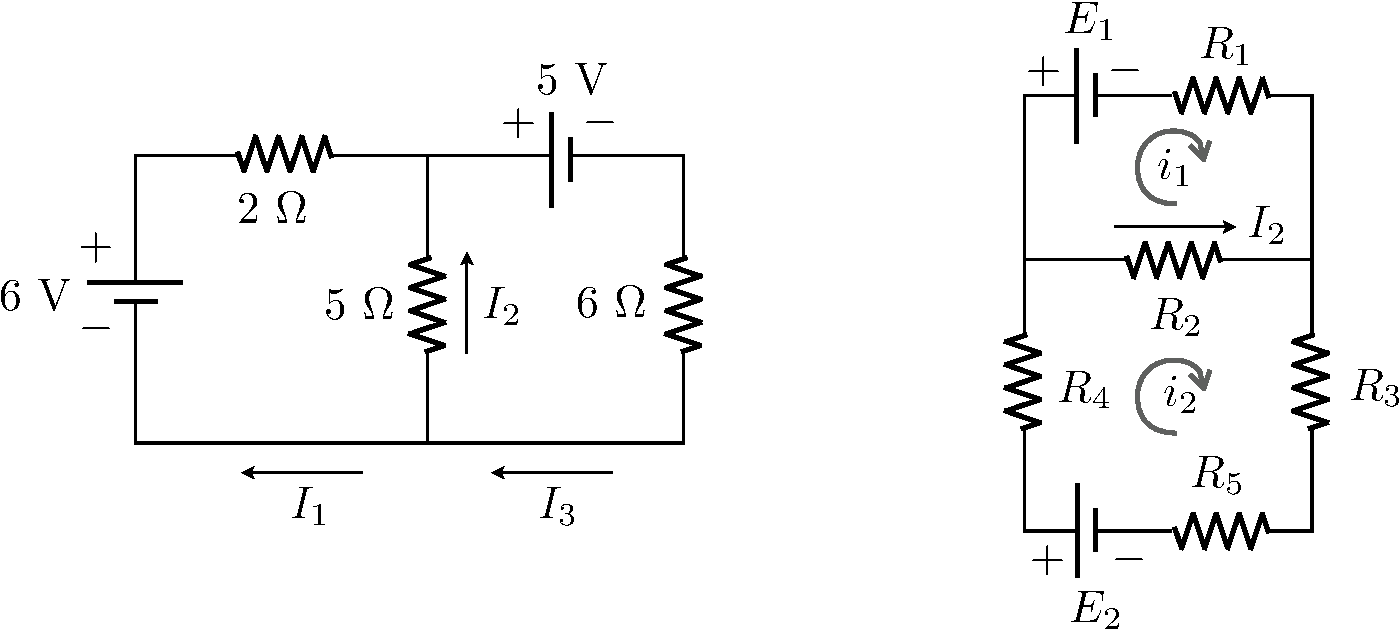
\includegraphics[width=5in]{3_netprob}}
%\hspace{5mm}
%\includegraphics[height=1.25in]{3_netprob2}}
\caption{Circuit diagrams for Problems~\ref{np3_1} (left) and 
\ref{np3_2} (right). 
\label{fig_netprob}}
\end{figure}

\begin{problem}
\label{2009_a5_3}
Consider the resistor network:

\begin{center}
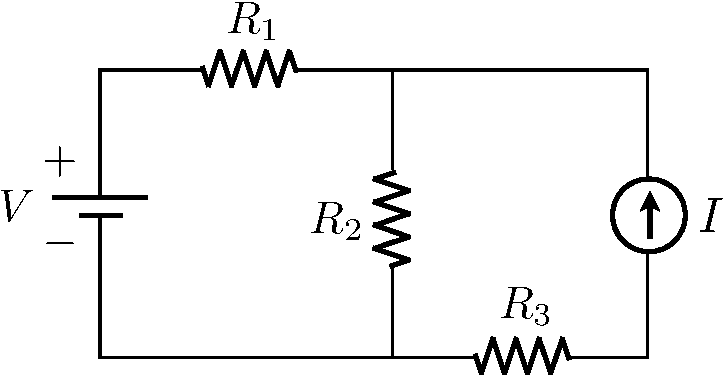
\includegraphics[height=1.25in]{3_fig5_3}
\end{center}
Given $R_1=3[\Omega]$, $R_2=1[\Omega]$, $R_3=4[\Omega]$, $V=26[V]$ and $I=2[A]$, answer the following questions:
\begin{enumerate}[a)]
\item What is the voltage drop through $R_3$?
\item What is the current flow through $R_2$?
\item What is the voltage drop through $R_1$?
\end{enumerate}
\end{problem}

\begin{problem}
\label{2009_a5_4}
Consider the following resistor network:

\begin{center}
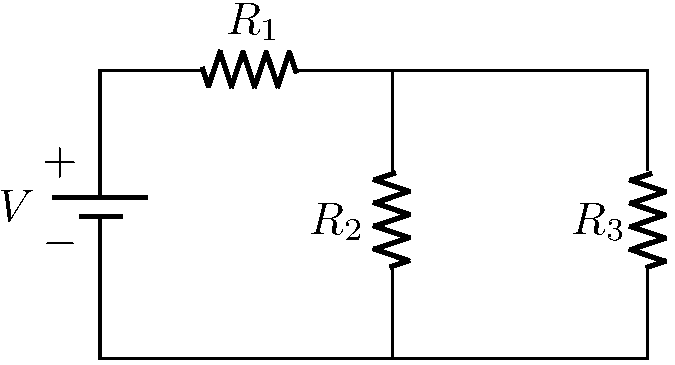
\includegraphics[height=1.25in]{3_fig5_1}
\end{center}
Suppose that $R_1=4[\Omega]$, $R_2=1[\Omega]$, $R_3=2[\Omega]$ and that the current flow through $R_3$ is $1.5[A]$. Solve the resistor network and answer the following questions:
\begin{enumerate}[a)]
\item What is the voltage drop across $R_3$?
\item What is the current flow through $R_2$?
\item What is the voltage drop through $V$?
\end{enumerate}
\end{problem}

\begin{problem}
\label{2009_a5_5}
Consider the following resistor network:

\begin{center}
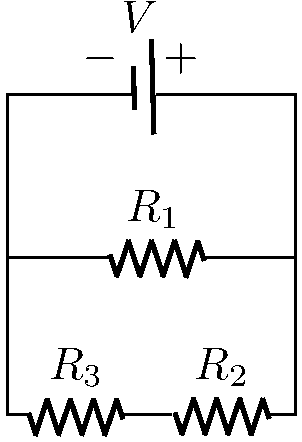
\includegraphics[height=1.25in]{3_fig5_2}
\end{center}
Suppose that $R_1=4[\Omega]$, $R_2=2[\Omega]$, $R_3=10[\Omega]$ and that $V=60[V]$. Solve the resistor network and answer the following questions:

\begin{enumerate}[a)]
\item What is the voltage drop through $R_2$?
\item What is the current flow through $R_1$?
\item What is the current flow through $R_3$?
\end{enumerate}
\end{problem}

\begin{problem}
\label{2009_a6_1}
Find the loop currents $i_1,i_2,i_3$ in the following network:

\centerline{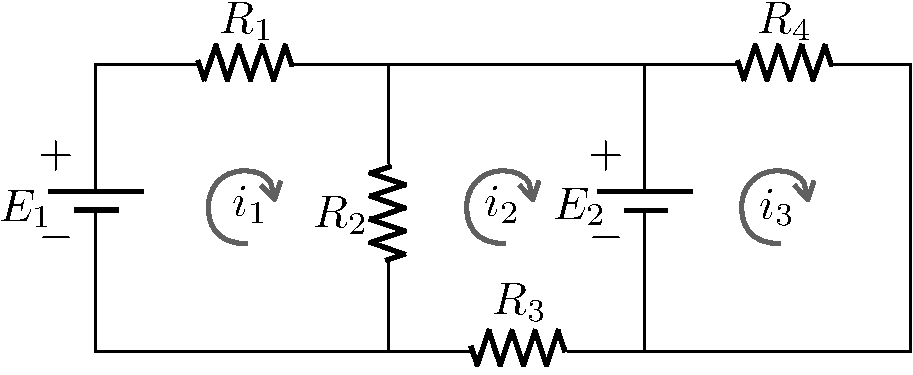
\includegraphics[height=1.5in]{3_fig6_1}}


where $R_1=1[\Omega]$, $R_2=3[\Omega]$, $R_3=5[\Omega]$, $R_4=2[\Omega]$, $E_1=10[V]$ and $E_2=4[V]$.
\end{problem}

\begin{problem}
\label{2009_a6_2}
Consider the following network:

\centerline{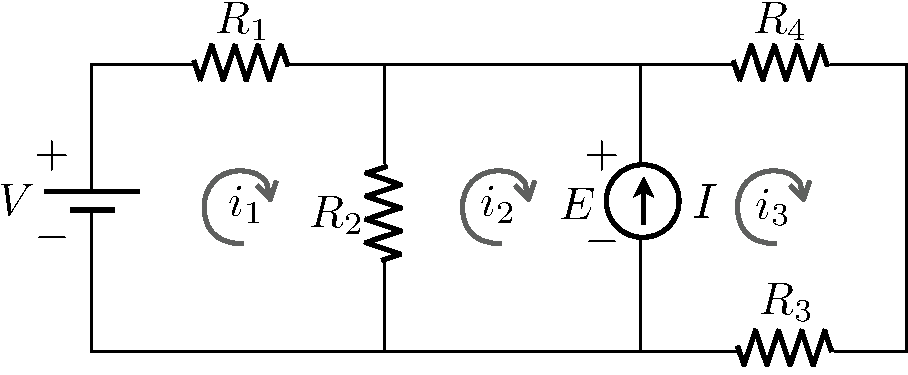
\includegraphics[height=1.5in]{3_fig6_2}}

where $R_1=1[\Omega]$, $R_2=2[\Omega]$, $R_3= 1 [\Omega]$, $R_4=1 [\Omega]$,
$V=25[V]$ and $I=3[A]$.
\begin{enumerate}[a)]
\item Set up and solve the linear system for the
loop currents $i_1,i_2,i_3$ and the voltage $E$ across the current source.
\item What is the voltage drop across $R_2$?
\item What is the current flow through the voltage source $V$?
\end{enumerate} 
\end{problem}

%\begin{problem}
%\label{2009_a6_3}
%Consider the resistor network:
%
%\centerline{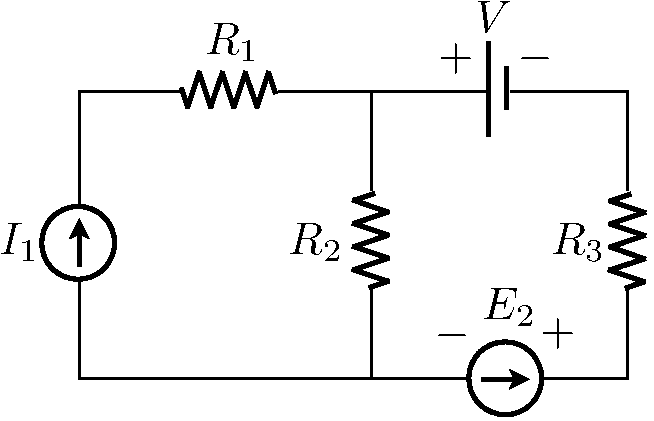
\includegraphics[height=1.5in]{3_fig6_3}}
%
%with $R_1=2[\Omega]$, $R_2=5[\Omega]$, $R_3=3[\Omega]$, $V=10[V]$, $I_1=3[A]$. Suppose that the voltage drop through $I_2$ is $E_2=5[V]$.
%\begin{enumerate}[a)]
%\item What is the current flow through $R_2$?
%\item What is the voltage drop through $I_1$?
%\item What is the current flow through $I_1$?
%\end{enumerate}
%\end{problem}

\begin{problem}
\label{op2_17}
If a circuit contains only resistors, then we can solve it completely 
using the ideas
of this section. 
Write down the linear equations satisfied by the currents in the
circuit shown in Figure~\ref{fig_circuit2}. 
In this diagram, the component on the far left is a voltage
source (battery). The voltage across the voltage source is always $E$.
\end{problem}

\begin{figure}
\centerline{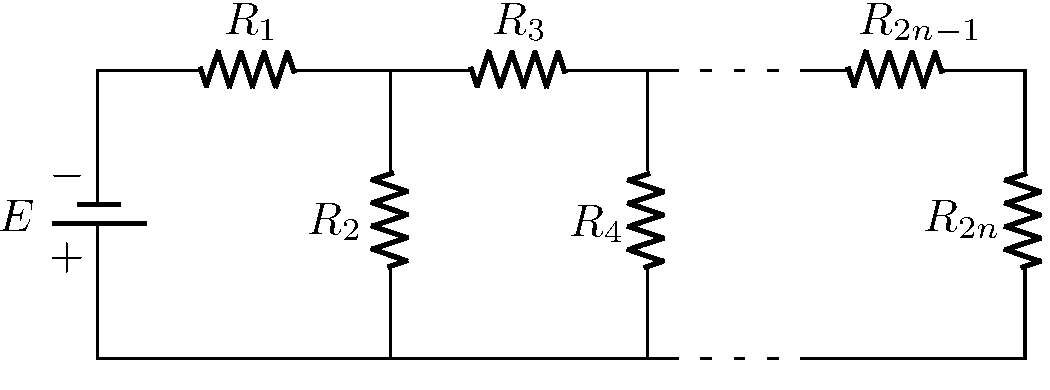
\includegraphics[height=1.5in]{3_circuit2}}
\caption{The circuit from Problem~\ref{op2_17}.
\label{fig_circuit2}}
\end{figure}

\section{Additional Topics}

\subsection{The Check Column}
\label{s:check} 

Ordinary arithmetic errors are a big problem when you do row operations
by hand. There is a technique called ``the check column'' (that is modeled
after the ``parity bit'' in computer hardware design) which provides a
very effective way to catch mechanical errors. Here is an example which
illustrates the technique:

\begin{example} 
The augmented matrix for the system of equations
\[
\begin{array}{rrrrrrr}
  2x_1&+&x_2&+&3x_3&=\,&1 \\
  4x_1&+&5x_2&+&7x_3&=\,&7\cr
  2x_1&-&5x_2&+&5x_3&=\,&-7\cr
 \end{array} 
\]
is
\[
\left[ \begin{array}{ccc|c} 2&1&3 & 1 \\  4&5&7&7 \\  2&-5 &5 & -7 \end{array} \right]
\]
To implement a ``check column'' you tack onto the right hand side of the 
augmented matrix an additional column. Each entry in this check column is 
the sum of all the entries in the row of the augmented matrix that is to 
the left of the check column entry. For example, the top entry in the check
column is $2+1+3+1=7$.
\[
\left[ \begin{array}{ccc|c} 2&1&3 & 1 \\  4&5&7&7 \\  2&-5 &5 & -7 \end{array} \right]
\begin{array}{c} 7 \\ 23 \\ -5 \end{array} 
\]
To use the check column you just perform the same row
operations on the check column as you do on the augmented matrix. After
each row operation you check that each entry in the check column is
still the sum of all the entries in the corresponding row of the augmented
matrix.

We now want to eliminate the $x_1$'s from equations (2) and (3). That is,
we want to make the first entries in rows 2 and 3 of the augmented matrix
zero. We can achieve this by subtracting two times row (1) from row (2) and 
subtracting row (1) from row (3).
\[
\begin{array}{c} (1) \\ (2)-2(1) \\ (3)-(1) \end{array} 
\left[ \begin{array}{ccc|c} 2&1&3 & 1 \\  0&3&1&5 \\  0&-6 &2 & -8 \end{array} \right]
\begin{array}{c} 7 \\ 9 \\ -12 \end{array} 
\]
Observe that the check column entry $9$ is the sum $0+3+1+5$ 
of the entries in the second row of the augmented matrix. If this were
not the case, it would mean that we made a mechanical error. Similarly
the check column entry $-12$ is the sum $0-6+2-8$.

We have now succeeded in eliminating all of the $x_1$'s from equations
(2) and (3). For example, row 2 now stands for the equation
\[
3x_2+x_3=5
\]
We next use equation (2) to eliminate all $x_2$'s from equation
(3).
\[
\begin{array}{c} (1) \\ (2) \\ (3)+2(2) \end{array} 
\left[ \begin{array}{ccc|c} 2&1&3 & 1 \\  0&3&1&5 \\  0& 0&4 & 2 \end{array} \right]
\begin{array}{c} 7 \\ 9 \\ 6 \end{array} 
\]
We can now easily solve (3) for $x_3$, substitute the result back into (2) and
solve for $x_2$ and so on:
\begin{eqnarray*}
(3) &\rightarrow & 4x_3 =2  \rightarrow x_3 = \frac{1}{2} \\
(2) &\rightarrow & 3x_2 +\frac{1}{2} =5  \rightarrow x_2 = \frac{3}{2} \\
(1) &\rightarrow & 2x_1 + \frac{3}{2} + 3 \times \frac{1}{2} =1  \rightarrow x_1 = -1
\end{eqnarray*}
This last step is called ``backsolving''.
\end{example} 

Note that there is an easy way to make sure that we have not made any mechanical
errors in deriving this solution --- just substitute the purported solution
$(-1,3/2,1/2)$ back into the original system:
\[
\begin{array}{rrrrrrr}
  2(-1)&+& \frac{3}{2} &+&3 \times \frac{1}{2} &=\,&1 \\
  4(-1)&+&5\times \frac{3}{2}&+&7 \times \frac{1}{2}&=\,&7\cr
  2(-1)&-&5\times \frac{3}{2} &+&5 \times \frac{1}{2}&=\,&-7\cr
 \end{array} 
\]
and verify that each left hand side really is equal to its corresponding
right hand side. However, if this test fails, all we would know is that we had made an error somewhere in the elimination process. The check column technique can identify the place where the error was made. 

\subsection{Quadratic Functions}

Let begin by recalling how we would find the minimum of a quadratic function in
one variable, namely a parabola given by $f(x) = a x^2 + bx + c$ as
shown in Figure~\ref{fig_parabola}. We simply find
the value of $x$ for which the derivative is zero, that is, we solve $f'(x)=0$.
Notice that since $f$ is quadratic, this is a linear equation
\[
2ax+b=0
\]
which is easily solved for $x=-b/2a$ (provided $a\ne 0$). 
So the minimum value is $f(-b/2a) = -b^2/(4a) + c$.

\begin{figure}
\centerline{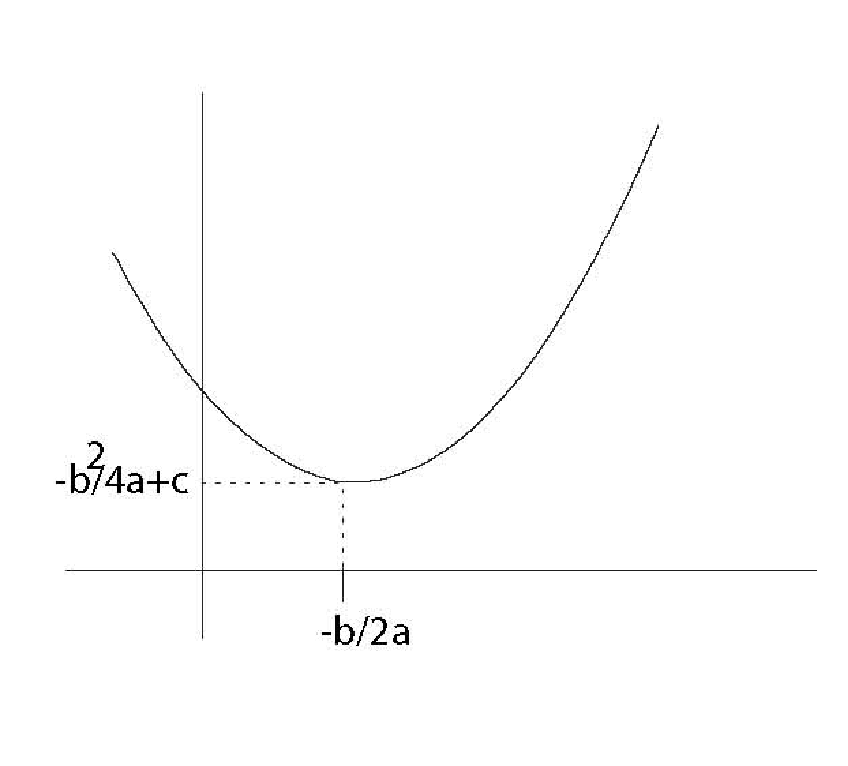
\includegraphics[height=1.5in]{3_parabola}}
\caption{The minimization of a quadratic function in one variable. 
\label{fig_parabola}}
\end{figure}

Of course, if $a$ is negative, then the parabola points downwards, and
we have found the maximum value, not the minimum value.

A quadratic function of two variables $x_1$ and $x_2$ is a function of the
form
\[
f(x_1,x_2)= ax_1^2 + 2bx_1x_2 + cx_2^2 + dx_1 + ex_2+f.
\]
(The $2$ in front of $b$ is just for convenience.) For what values of
$x_1$ and $x_2$ is $f(x_1,x_2)$ the smallest? Just like with the parabola in
one variable, there may be no such values. It could be that $f$ has a maximum
instead, or that $f$ has what is called a {\em saddle point}. However if $f$ does have
a minimum, the procedure described below is guaranteed to find it. (If $f$
has a maximum or saddle point, the procedure will find these points instead.)

The idea behind finding the minimum is simple. Suppose that $x_1$ and
$x_2$ are the values for which $f(x_1,x_2)$ is smallest. Then the function
$g(s) = f(x_1+s,x_2)$ must have a minimum at $s=0$. So $g'(0)=0$. But
\begin{eqnarray*}
g'(s) &=& {{d}\over{ds}}f(x_1+s,x_2) \\
&=&{{d}\over{ds}}a(x_1+s)^2 + 2b(x_1+s)x_2 + cx_2^2 +
d(x_1+s) + ex_2+f \\
&=& 2a(x_1+s) + 2bx_2 + d
\end{eqnarray*}
so that the condition is
\[
g'(0) = 2ax_1 + 2bx_2 + d = 0.
\]
Notice that this expression can be obtained by holding $x_2$ fixed and
differentiating with respect to $x_1$. It is called the partial derivative of
$f$ with respect to $x_1$ and is denoted ${{\PA f}\over{\PA x_1}}$.

The same argument can be applied to $h(s)=f(x_1,x_2+s)$ (or 
${{\PA f}\over{\PA x_2}}$.)
This yields
\[
h'(0) = {{\PA f(x_1,x_2)}\over{\PA x_2}} = 2bx_1 + 2cx_2 + e = 0.
\]

Therefore we conclude that the pair of values $x_1$ and $x_2$ at which
$f$ achieves its minimum satisfy the system of linear equations
\[
\matrix{
2ax_1 &+ 2bx_2 &= -d\cr
2bx_1 &+ 2cx_2 &= -e\cr
}
\]
This is a $2$ by $2$ system with augmented matrix
\[
\left[\matrix{
2a&2b\cr
2b&2c\cr
}\right.\left|\matrix{
-d\cr -e\cr
}\right]
\]

This is easily generalized to $n$ variables. 
In this case the quadratic function is given by
\[
f(x_1,x_2,\ldots,x_n)=\sum_{i=1}^n\sum_{j=1}^n a_{i,j}x_ix_j
+\sum_{i=1}^nb_ix_i+c
\]
To see this is the same, let us expand out the first term when $n=2$. Then
\begin{eqnarray*}
\sum_{i=1}^n\sum_{j=1}^n a_{i,j}x_ix_j
&=&a_{1,1}x_1x_1+a_{1,2}x_1x_2+a_{2,1}x_2x_1+a_{2,2}x_2x_2 \\
&=& a_{1,1}x_1^2+(a_{1,2}+a_{2,1})x_1x_2+a_{2,2}x_2^2 
\end{eqnarray*}
So this is just the same as before with $a_{1,1}=a$, $a_{1,2}+a_{2,1}=2b$ and
$a_{2,2}=c$. Notice that we might as well assume that $a_{i,j}=a_{j,i}$, since
replacing both $a_{i,j}$ and $a_{j,i}$ with $(a_{1,2}+a_{2,1})/2$ doesn't change
$f$.

If this function $f$ has a minimum we can find it by generalizing the procedure
above. In other words we try to find values of $x_1,\ldots,x_n$ for which
$\PA f/\PA x_1 = \PA f/\PA x_2=\cdots=\PA f/\PA x_n=0$. This leads to a system
of $n$ linear equations whose associated augmented matrix is
\[
\left[\matrix{
2a_{1,1}&2a_{1,2}&\ldots&2a_{1,n}\cr
2a_{2,1}&2a_{2,2}&\ldots&2a_{2,n}\cr
\vdots&\vdots&&\vdots\cr
2a_{n,1}&2a_{n,2}&\ldots&2a_{n,n}\cr
}\right.\left|\matrix{
-b_1\cr -b_2\cr \vdots\cr -b_n\cr
}\right]
\]

\subsection{Least squares fit}

As a first application let us  consider the problem of finding the ``best''
straight line going through a collection of data points $(x_1,y_1),
(x_2,y_2),\ldots,(x_n,y_n)$. (Careful! the  $x_i$'s are not the unknowns in this
problem, but rather the known fixed data points, together with the $y_i$'s.)
Consider Figure~\ref{fig_leastsquares}. 
Which straight line fits best? There is no one answer. One can measure how good the fit of
a straight line is in various ways. However the following way of measuring the
fit results in a problem that is easy to solve.

\begin{figure}
\centerline{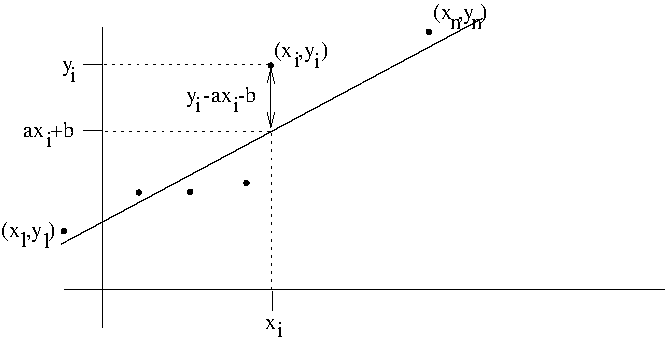
\includegraphics[height=1.5in]{3_leastsquares}}
\caption{Fitting a line through data.
\label{fig_leastsquares}}
\end{figure}

Each line is given by an equation $y=ax+b$. So the variables in this problem are
$a$ and $b$. We want to find the values of $a$ and $b$ that give the best
fitting line. The vertical distance between the point $(x_i,y_i)$ and the line
is given by $|y_i-ax_i-b|$. We will take as a measure of the fit, the square of
this quantity, added up over all the data points. So
\begin{eqnarray*}
f(a,b) &= &\sum_i (y_i-ax_i-b)^2 \\
&=&\sum_i\left(y_i^2+x_i^2a^2+b^2 -2x_iy_ia-2y_ib+2x_iab\right) \\
&=&\left(\sum_i x_i^2\right)a^2 +2\left(\sum_i x_i\right)ab + nb^2
-2\left(\sum_i x_iy_i\right)a -2\left(\sum_i y_i\right)b
+\left(\sum_i y_i^2\right)
\end{eqnarray*}
Here we used that $(\sum_i 1)=n$, the number of points.
Therefore the linear equations we must solve for $a$ and $b$ are
\[
\left[\matrix{
2\left(\sum_i x_i^2\right)&2\left(\sum_i x_i\right)\cr
2\left(\sum_i x_i\right)&2n\cr
}\right.\left|\matrix{
2\left(\sum_i x_iy_i\right)\cr 2\left(\sum_i y_i\right)\cr
}\right]
\]
We could solve these equations numerically in each particular case, but since
its just a $2$ by $2$ system we can also write down the answer explicitly.
In fact, the solution to
\[
\left[\matrix{
A&B\cr
C&D\cr
}\right.\left|\matrix{
E\cr F\cr
}\right]
\]
is
\[
\left[\matrix{{{DE-BF}\over{AD-BC}}\cr
{{AF-CE}\over{AD-BC}}\cr}\right],
\]
provided $AD-BC\ne0$,
as you may check directly, or derive using a sequence of row transformations.
So in this case
\begin{eqnarray*}
a&=&{{n(\sum x_iy_i)-(\sum x_i)(\sum y_i)}\over{n(\sum x_i^2)-
   (\sum x_i)^2}} \\
b&=&{{(\sum x_i^2)(\sum y_i)-(\sum x_i)(\sum x_iy_i)}
   \over{n(\sum x_i^2)-(\sum x_i)^2}} \\
\end{eqnarray*}

\begin{example}
\label{ex_lsfit}
Suppose we want to find the best straight line through
the points $(1,1)$, $(2,2)$, $(2,3)$, $(3,3)$ and $(3,4)$. 
{\rm Calculate
\[
\matrix{
\sum 1 &= n&= 5\cr
\sum x_i &= 1+2+2+3+3 &= 11\cr
\sum y_i &= 1+2+3+3+4 &= 13\cr
\sum x_i^2&= 1+4+4+9+9 &= 27\cr
\sum y_i^2&= 1+4+9+9+16 &= 39\cr
\sum x_iy_i&=1+4+6+9+12 &= 32\cr
}
\]
so
\[
a = (5\cdot 32-11\cdot 13)/(5\cdot 27-11^2) = 17/14 = 1.214\ldots
\]
and
\[
b = (27\cdot 13-11\cdot 32)/(5\cdot 27-11^2) = -1/14 = -0.0714\ldots
\]
The result is shown in Figure~\ref{fig_lsqeg}.}
\end{example}

\begin{figure}
\centerline{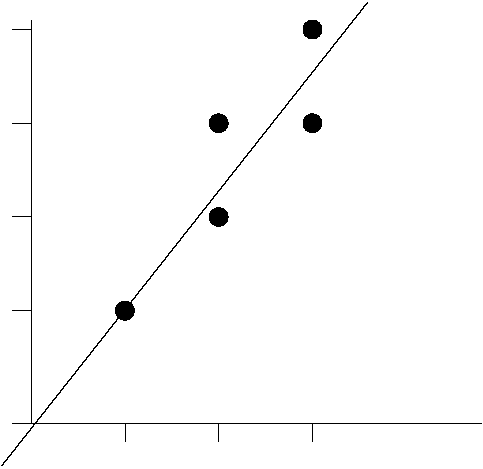
\includegraphics[height=1.5in]{3_lsqeg}}
\caption{The solution in Example~\ref{ex_lsfit}.
\label{fig_lsqeg}}
\end{figure}

\subsection{Equilibrium configuration of hanging weights and springs}

Consider the problem of $n$ vertically hanging weight connected by springs.
What is the equilibrium configuration? We can solve this problem by calculating
the total potential energy of the system. The equilibrium configuration
minimizes the total potential energy.
A diagram of the setup is shown in Figure~\ref{fig_springs}. 
Our goal is to compute the numbers $x_1$,
$\ldots$, $x_n$. In the diagram $n=3$.

\begin{figure}
\centerline{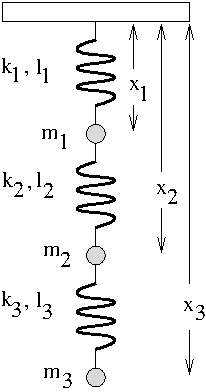
\includegraphics[height=1.5in]{3_springs}}
\caption{Equilibrium configuration of springs.
\label{fig_springs}}
\end{figure}

There are two sources of potential energy. One is the potential energy stored in
the spring. This is equal to $k s^2/2$, where $k$ is the spring constant that
measures the stiffness of the spring, and $s$ is the amount that the spring has
been stretched from its natural length. In our problem, suppose that the
spring constant of the $i$th spring is $k_i$ and its natural
length is $l_i$. Then the potential energy stored in the $i$th spring
is $k_i(x_{i}-x_{i-1}-l_i)^2/2$. To make this formula work out correctly for the
first spring we set $x_0=0$.

The other source of potential energy is gravity. The gravitational potential
energy of the $i$th weight is $-m_igx_i$. The reason for the minus sign is that
we are measuring distances downward.

Thus the total potential energy in the system for $n$ weights is the function
\[
f(x_1,x_2,\ldots, x_n) = \sum_{i=1}^n {{k_i}\over{2}}(x_{i}-x_{i-1}-l_i)^2 - m_igx_i.
\]
When $n=3$ this becomes
\[
f(x_1,x_2,x_3) = {{k_1}\over{2}}(x_1-l_1)^2 + {{k_2}\over{2}}(x_2-x_1-l_2)^2
+{{k_3}\over{2}}(x_3-x_2-l_3)^2 -m_1gx_1-m_2gx_2-m_3gx_3
\]
This is a quadratic function, so we know how to find the minimum. The equations
are obtained by taking partial derivatives: To get the first equation we hold
$x_2$ and $x_3$ fixed and differentiate with respect to $x_1$ and so on. Thus
the equations are
\begin{eqnarray*}
k_1(x_1-l_1) - k_2(x_2-x_1-l_2) - m_1g &=&0 \\
k_2(x_2-x_1-l_2) - k_3(x_3-x_2-l_3) - m_2g &=&0 \\
k_3(x_3-x_2-l_3) -m_3g&=&0
\end{eqnarray*}
The augmented matrix for this system is
\[
\left[\matrix{
k_1+k_2&-k_2&0\cr
-k_2&k_2+k_3&-k_3\cr
0&-k_3&k_3\cr
}\right.\left|\matrix{
m_1g+k_1l_1-k_2l_2\cr m_2g+k_2l_2-k_3l_3\cr m_3g+k_3l_3\cr
}\right]
\]

\begin{example}
Suppose that the spring constants are $k_1=1$, $k_2=2$ and $k_3=1$. The
masses are all equal to $1$, $g=10$ and the natural length of the springs
is $1$ for all springs (in appropriate units). Find the equilibrium
configuration.
{\rm We must solve
\[
\left[\matrix{
3&-2&0\cr
-2&3&-1\cr
0&-1&1\cr
}\right.\left|\matrix{
9\cr 11\cr 11\cr
}\right]
\]
Gaussian elimination gives
\[
\left[\matrix{
3&-2&0\cr
0&-1&1\cr
0&0&2\cr
}\right.\left|\matrix{
9\cr 11\cr 106\cr
}\right]
\]
which can be solved to give $x_1=31$, $x_2=42$, $x_3=53$.}
\end{example}

\subsection{Problems}

\begin{problem}
\label{op2_13}
Find the ``best'' straight line going through the points
$(1,1)$, $(2,1)$, $(2,3)$, $(3,4)$, $(3,5)$ and $(4,4)$.
\end{problem}

\begin{problem}
\label{op2_14}
Consider the problem of finding the parabola $y=ax^2+bx+c$ that best fits the n
data points $(x_1,y_1)\ldots (x_n,y_n)$. Derive the system of three linear
equations which determine $a$, $b$ and $c$. (You need not solve solve them!)
\end{problem}

\begin{problem}
\label{op2_15}
Write down the augmented matrix for a system of $n$ weights and springs.
\end{problem}

\begin{problem}
\label{op2_16}
Write down the system of equations you would have to solve if there are
$5$ identical springs with $k_i=1$ and $l_i=1$ and five weights
with $m_1=1$, $m_2=2$, $m_3=3$, $m_4=4$, and $m_5=5$.
\end{problem}


\section{Solutions to Chapter Problems}

%%%%%%%%%%%%%%%%%%%%%%%%%%%%%%%%%%%%%%%%%%%%%%%%%%%%%%%%%%%%%%%%%%%%%%%%%%%%%%%%
\vspace{2mm}
\noindent {\bf Solution \ref{2009_a3_5}}
The augmented matrix is
$$
A = \left[\begin{array}{ccc|c}
  1 & -2 & 3 & 6\\
	4 & -5 & -6 & 7\\
	8 & 9 & 10 & 11
\end{array}\right]
$$


%%%%%%%%%%%%%%%%%%%%%%%%%%%%%%%%%%%%%%%%%%%%%%%%%%%%%%%%%%%%%%%%%%%%%%%%%%%%%%%%
\noindent {\bf Solution \ref{op2_1}}
Here is the sequence of systems of equations you would get:
\[
\matrix{
x_1&+&x_2&+&x_3&=&6\cr
x_1&-&x_2&+&x_3&=&0\cr
2x_1&+&x_2&-&8x_3&=&-11\cr
}
\]
%
\[
\matrix{
x_1&+&x_2&+&x_3&=&6\cr
&-&	2x_2&&	&=&	-6\cr
2x_1&+&x_2&-&8x_3&=&-11\cr
}
\]
%
\[
\matrix{
x_1&+&	x_2&+&	x_3&=&	6\cr
&-&	2x_2&&	&=&	-6\cr
&-&	x_2&-&	10x_3&=&	-23\cr
}
\]
%
\[
\matrix{
x_1&+&	x_2&+&	x_3&=&	6\cr
&&	x_2&&	&=&	3\cr
&-&	x_2&-&	10x_3&=&	-23\cr
}
\]
%
\[
\matrix{
x_1&+&	x_2&+&	x_3&=&	6\cr
&&	x_2&&	&=&	3\cr
&&	&-&	10x_3&=&	-20\cr
}
\]
So $x_3=2$, $x_2=3$ and $x_1=1$.

%%%%%%%%%%%%%%%%%%%%%%%%%%%%%%%%%%%%%%%%%%%%%%%%%%%%%%%%%%%%%%%%%%%%%%%%%%%%%%%%
\vspace{2mm}
\noindent {\bf Solution \ref{matlab_op2_1}}
\begin{verbatim}
A = [1, 1, 1, 6; 1, -1, 1, 0; 2, 1, -8, -11]
A(2,:) = A(2,:) - A(1,:)
A(3,:) = A(3,:) - 2*A(1,:)
A(2,:) = -A(2,:)/2
A(3,:) = A(3,:) + A(2,:)
A(3,:) = -A(3,:)/10
\end{verbatim}
We get the same solution as in the pen-and-paper version in problem \ref{op2_1}.

%%%%%%%%%%%%%%%%%%%%%%%%%%%%%%%%%%%%%%%%%%%%%%%%%%%%%%%%%%%%%%%%%%%%%%%%%%%%%%%%
\vspace{2mm}
\noindent {\bf Solution \ref{2009_a3_4}}
Perform the sequence of operations to finally end up with the system
\begin{eqnarray*}
  2x_3 &=& 4 \\
	3x_1 - 3x_2 + 3x_3 &=& 30 \\
	9x_1 \hspace{27pt} + 2x_3 &=& 26.
\end{eqnarray*}
%
Hence, $x_1 = 22/9$, $x_2 = -50/9$, and $x_3 = 2$.


%%%%%%%%%%%%%%%%%%%%%%%%%%%%%%%%%%%%%%%%%%%%%%%%%%%%%%%%%%%%%%%%%%%%%%%%%%%%%%%%
\vspace{2mm}
\noindent {\bf Solution \ref{2009_a3_3}}
We want to solve the system
\begin{eqnarray*}
  2x_1 + x_2 &=& 5 \\
	3x_1 + 5x_2 &=& -10. \\
\end{eqnarray*}
We shall use the method of substitution.

From the first equation, we solve for $x_2$:
$$x_2 = 5 - 2x_1$$
We then substitute it into the second equation:
$$3x_1 + 5(5 - 2x_1) = -10$$.
We now have a decoupled equation, and the solution is $x_1 = 5$, $x_2 = -5$.

%%%%%%%%%%%%%%%%%%%%%%%%%%%%%%%%%%%%%%%%%%%%%%%%%%%%%%%%%%%%%%%%%%%%%%%%%%%%%%%%
\vspace{2mm}
\noindent {\bf Solution \ref{op2_2}}
The first equation reads $x_1=3$. The second reads $x_1-x_2=3$, or $3-x_2=3$, or
$x_2=0$. The third reads $2x_1+x_2-8x_3=-4$, or $6+0-8x_3=-4$ or $x_3=5/4$. 

%%%%%%%%%%%%%%%%%%%%%%%%%%%%%%%%%%%%%%%%%%%%%%%%%%%%%%%%%%%%%%%%%%%%%%%%%%%%%%%%
\vspace{2mm}
\noindent {\bf Solution \ref{op2_3}}
The last equation gives $x_4=2$ and the second last one $x_3=2$. Then we have to
introduce a parameter $x_2-s$ and the we find that $x_1=-5-2s$ Thus
$\xx=\left[\matrix{-5\cr 0\cr 2\cr 2\cr}\right] + s \left[\matrix{-2\cr 1\cr
0\cr 0\cr}\right]$
In the second system, we have to introduce a parameter right off the bat. So
$x_4=s_1$ and $x_3=4-s_1$. Moving up one row, we have to introduce another
parameter $x_2=s_2$ and then $x_1=1-2s_2-(4-s_1)-2s_1=-3-s_1-2s_2$
so $\xx=\left[\matrix{-3\cr 0\cr 4\cr 0\cr}\right] + s_1 \left[\matrix{-1\cr 0\cr
-1\cr 1\cr}\right] + s_2 \left[\matrix{-2\cr 1\cr
0\cr 0\cr}\right]$
The third system is just the same. The extra rows of zeros have no effect.

%%%%%%%%%%%%%%%%%%%%%%%%%%%%%%%%%%%%%%%%%%%%%%%%%%%%%%%%%%%%%%%%%%%%%%%%%%%%%%%%
\vspace{2mm}
\noindent {\bf Solution \ref{2009_a4_3}}
Perform the following sequence of row operations:
\begin{enumerate}[i)]
\item $(2,:) = (2,:) - (1,:)$
\item $(3,:) = (3,:) - (1,:)$
\item $(3,:) = (3,:) + 2(2,:)$
\item $(4,:) = (4,:) - 3(2,:)$
\item $(4,:) = (4,:) + (3,:)$,
\end{enumerate}
in order to get the reduced row echelon form (RREF)
$$
\left[\begin{array}{cccc|c}
     1 & 2 & 2 & 2 & 1 \\
		 0 & 1 & -3 & 1 & -2\\
		 0 & 0 & -7 & 1 & 0\\
		 0 & 0 & 0 & 0 & 0
      \end{array}\right].
$$
Thus, we have that the rank of the augmented matrix, which is the same as the rank of the unaugmented matrix is $r=3$, while the number of unknowns is $n=4$. Therefore, the system has infinitely many solutions, that can be represented as the general solution
$$
\xx = \qq + s\aa,
$$
where $s$ is any real number, $\qq = (q_1,q_2,q_3,q_4)$ is any particular solution of the original system, and $\aa = (a_1, a_2, a_3, a_4)$ is any non-zero solution of the corresponding homogeneous system.

From the row echelon form we can see that $\qq$ has to satisfy $- 7q_3 + q_4 = 0$. Let $q_4 = 7$, then $q_3 = 1$. For the other two $q$ values we have
\begin{eqnarray*}
  q_2 &=& -2 + 3q_3 - q_4 = -6 \\
	q_1 &=& 1 - 2q_2 - 2q_3 - 2q_4 = -3.
\end{eqnarray*}
Hence, we have that $\qq = (-3, -6, 1, 7)$.

Now, to find $\aa$, the homogenous row echelon form is
$$
\left[\begin{array}{cccc|c}
     1 & 2 & 2 & 2 & 0 \\
		 0 & 1 & -3 & 1 & 0\\
		 0 & 0 & -7 & 1 & 0\\
		 0 & 0 & 0 & 0 & 0
      \end{array}\right].
$$
Thus, $\aa$ has to satisfy $-7a_3 + a_4 = 0$. Take $a_4 = 7$, then $a_3 = 1$.

From the second row we have that $a_2 = 3a_3 - a_4 = -4$, and from the first row we get that $a_1 = -2a_2 - 2a_3 - 2a_4 = -8$. So $\aa = (-8, -4, 1, 7)$, and a general form of the solution is
$$
\xx = \left[\begin{array}{c} -3 \\ -6 \\ 1 \\ 7 \end{array}\right] +
s\left[\begin{array}{c} -8 \\ -4 \\ 1 \\ 7 \end{array}\right]
$$

%%%%%%%%%%%%%%%%%%%%%%%%%%%%%%%%%%%%%%%%%%%%%%%%%%%%%%%%%%%%%%%%%%%%%%%%%%%%%%%%
\vspace{2mm}
\noindent {\bf Solution \ref{2009_a4_1}}
Perform the following sequence of row operations
\begin{enumerate}[i)]
\item $(2,:) = (2,:) - 3(1,:)$
\item $(4,:) = (4,:) - 2(1,:)$
\item $(4,:) = (4,:) + 2(3,:)$
\item $(3,:) \leftrightarrow (2,:)$
\item $(4,:) \leftrightarrow (3,:)$
\item $(4,:) = (4,:) - \frac{3}{2}(3,:)$,
\end{enumerate}
to transform the augmented matrix into the reduced row echelon form
$$
\left[\begin{array}{cccc|c}
     1 & 2 & 2 & -7 & 20 \\
		 0 & 6 & 0 & -6 & -10\\
		 0 & 0 & -6 & 0  & -30\\
		 0 & 0 & 0 & 16 & -30
      \end{array}\right].
$$
We can now solve the system starting from the bottom:
\begin{eqnarray*}
x_4 &=& -\frac{30}{16} = -\frac{15}{8} \\
x_3 &=& \frac{-30}{-6} = 5 \\
x_2 &=& \frac{-10 + 6x_4}{6} = -\frac{85}{24} \\
x_1 &=& 20 - 2x_2 - 2x_3 + 7x_4 = \frac{95}{24}
\end{eqnarray*}

%%%%%%%%%%%%%%%%%%%%%%%%%%%%%%%%%%%%%%%%%%%%%%%%%%%%%%%%%%%%%%%%%%%%%%%%%%%%%%%%
\vspace{2mm}
\noindent {\bf Solution \ref{op2_4}}
The matrix 
\[
\left[
\begin{array}{ccc}
1&-2&3 \\
2&-3&2 \\
3&2&-4 
\end{array} \right| \left.
\begin{array}{c}
2 \\ 2 \\ 9
\end{array}
\right]
\]
reduces to
\[
\left[
\begin{array}{ccc}
1&-3&3 \\
0&1&4 \\
0&0&19
\end{array} \right| \left.
\begin{array}{c}
2 \\ -2 \\ 19
\end{array}
\right]
\]
which has as solution
$x_1=3$, $x_2=2$, $x_3=1$.
%%%%%%%%%%%%%%%%%%%%%%%%%%%%%%%%%%%%%%%%%%%%%%%%%%%%%%%%%%%%%%%%%%%%%%%%%%%%%%%%

\vspace{2mm}
\noindent {\bf Solution \ref{op2_5}}
The matrix 
\[
\left[
\begin{array}{ccc}
2&1&-1 \\
1&-2&-2 \\
-1&12&8
\end{array} \right| \left.
\begin{array}{c}
6 \\ 1 \\ 7
\end{array}
\right]
\]
reduces to
\[
\left[
\begin{array}{ccc}
2&1&-1 \\
0&-5/2&-3/2 \\
0&0&0
\end{array} \right| \left.
\begin{array}{c}
6 \\ -2 \\ 0
\end{array}
\right]
\]
which has as solution
$x_1=13/5+4s/5$, $x_2=4/5-3s/5$, $x_3=s$.
%%%%%%%%%%%%%%%%%%%%%%%%%%%%%%%%%%%%%%%%%%%%%%%%%%%%%%%%%%%%%%%%%%%%%%%%%%%%%%%%

\vspace{2mm}
\noindent {\bf Solution \ref{op2_6}}
The matrix 
\[
\left[
\begin{array}{ccc}
1&2&4 \\
1&1&3 \\
2&5&9
\end{array} \right| \left.
\begin{array}{c}
1 \\ 2 \\ 1
\end{array}
\right]
\]
reduces to
\[
\left[
\begin{array}{ccc}
1&2&4 \\
0&-1&-1 \\
0&0&0
\end{array} \right| \left.
\begin{array}{c}
1 \\ 1 \\ 0
\end{array}
\right]
\]
Thus , setting $x_3=s$, we obtain $x_2 = -1-s$ and $x_1=3-2s$.

%%%%%%%%%%%%%%%%%%%%%%%%%%%%%%%%%%%%%%%%%%%%%%%%%%%%%%%%%%%%%%%%%%%%%%%%%%%%%%%%
\vspace{2mm}
\noindent {\bf Solution \ref{op2_7}}
The matrix 
\[
\left[
\begin{array}{ccc}
1&2&4 \\
1&1&3 \\
2&5&9
\end{array} \right| \left.
\begin{array}{c}
1 \\ 2 \\ 3
\end{array}
\right]
\]
reduces to
\[
\left[
\begin{array}{ccc}
1&2&4 \\
0&-1&-1 \\
0&0&0
\end{array} \right| \left.
\begin{array}{c}
1 \\ 1 \\ 2
\end{array}
\right]
\]
which has no solutions.
\bigskip

%%%%%%%%%%%%%%%%%%%%%%%%%%%%%%%%%%%%%%%%%%%%%%%%%%%%%%%%%%%%%%%%%%%%%%%%%%%%%%%%
\vspace{2mm}
\noindent {\bf Solution \ref{op2_8}}
The matrix 
\[
\left[
\begin{array}{cccc}
3&1&-1&2 \\
2&-2&5&-7 \\
-4&-4&7&-11
\end{array} \right| \left.
\begin{array}{c}
7 \\ 1 \\-13 
\end{array}
\right]
\]
reduces to
\[
\left[
\begin{array}{cccc}
3&1&-1&2 \\
0&-8/3&17/3&-25/3 \\
0&0&0&0
\end{array} \right| \left.
\begin{array}{c}
7 \\ -11/3 \\ 0
\end{array}
\right]
\]
which has as solution
$x_1=15/8-3s_1/8+3s_2/8$, $x_2=11/8+17s_1/8-25s_2/8$, $x_3=s_1$, $x_4=s_2$.

%%%%%%%%%%%%%%%%%%%%%%%%%%%%%%%%%%%%%%%%%%%%%%%%%%%%%%%%%%%%%%%%%%%%%%%%%%%%%%%%
\vspace{2mm}
\noindent {\bf Solution \ref{op2_9}}
Probably the easiest way to do this problem is to think geometrically. This
system of equations describes the intersection of two lines. The lines will
intersect in a single point if they are not parallel. This will happen exactly
when the two vectors $[a,b]$ and $[c,d]$ are not parallel. Recall that this can
be tested using the determinant. So the equations have a unique solution exactly
when $\det\left[\matrix{a&b\cr c&d\cr}\right]=ad-bc\ne0$.

%%%%%%%%%%%%%%%%%%%%%%%%%%%%%%%%%%%%%%%%%%%%%%%%%%%%%%%%%%%%%%%%%%%%%%%%%%%%%%%%
\vspace{2mm}
\noindent {\bf Solution \ref{2009_a4_2}}
Perform the following sequence of row operations:
\begin{enumerate}[i)]
\item $(2,:) = (2,:) - 4(1,:)$
\item $(3,:) = (3,:) + 4(1,:)$
\item $(3,:) = (3,:) + \frac{5}{3}(3,:)$
\end{enumerate}
to get the reduced row echelon matrix
$$
\left[\begin{array}{ccc|c}
     1 & 2 & 0 & 7 \\
		 0 & 0 & 6 & -18\\
		 0 & 0 & 0  & 139\\
      \end{array}\right].
$$
The last equation says $0=139$, which cannot happen, therefore this linear system has \textbf{zero} solutions.

%%%%%%%%%%%%%%%%%%%%%%%%%%%%%%%%%%%%%%%%%%%%%%%%%%%%%%%%%%%%%%%%%%%%%%%%%%%%%%%%
\vspace{2mm}
\noindent {\bf Solution \ref{matlab_2009_a4_2}}
The script is the following:
\begin{verbatim}
for a = 1:10
A = [1 2 4 7; 4 1 3 2; 0 5 9 a];
rref(A)
end
\end{verbatim}
If the value of $a$ changes linearly, then the solution to $x_1$ (or for that matter, of $x_2$ and $x_3$ too) changes linearly with $a$.

%%%%%%%%%%%%%%%%%%%%%%%%%%%%%%%%%%%%%%%%%%%%%%%%%%%%%%%%%%%%%%%%%%%%%%%%%%%%%%%%
\vspace{2mm}
\noindent {\bf Solution \ref{2009_a4_4}}
Perform the following sequence of row operations:
\begin{enumerate}[i)]
\item $(2,:) = (2,:) + (1,:)$
\item $(3,:) = (3,:) - (2,:)$
\end{enumerate}
to get the reduced row echelon matrix
$$
\left[\begin{array}{cccc|c}
     1 & 0 & 1 & 0 & 10 \\
		 0 & 1 & 2 & 1 & 14\\
		 0 & 0 & 0 & 0 & 0\\
      \end{array}\right].
$$
Thus the row echelon form for the corresponding homogeneous system is
$$
\left[\begin{array}{cccc|c}
     1 & 0 & 1 & 0 & 0 \\
		 0 & 1 & 2 & 1 & 0\\
		 0 & 0 & 0 & 0 & 0\\
      \end{array}\right].
$$
Let $\qq$ be any solution to the original system. For example, check that $\qq = (9,11,1,1)$ solves the system.

Now, let $\aa_1$ and $\aa_2$ be any two linearly independent vectors which solve the corresponding homogeneous system. For example, check that $\aa_1 = (1,1,-1,1)$, and $\aa_2 = (1,-1,-1,3)$ are two linearly independent vectors, which solve the homogeneous system.

Thus, one representation for the solutions of the system is
$$
\xx = \left[\begin{array}{c} 9 \\ 11 \\ 1 \\ 1 \end{array}\right] +
s_1\left[\begin{array}{c} 1 \\ 1 \\ -1 \\ 1 \end{array}\right] + s_2\left[\begin{array}{c} 1 \\ -1 \\ -1 \\ 3 \end{array}\right].
$$

%%%%%%%%%%%%%%%%%%%%%%%%%%%%%%%%%%%%%%%%%%%%%%%%%%%%%%%%%%%%%%%%%%%%%%%%%%%%%%%%
\vspace{2mm}
\noindent {\bf Solution \ref{op2_11}}
The general solution is $[4,0,3,0]+s_1[-1,1,0,0]+s_2[0,0,-2,1]$.

%%%%%%%%%%%%%%%%%%%%%%%%%%%%%%%%%%%%%%%%%%%%%%%%%%%%%%%%%%%%%%%%%%%%%%%%%%%%%%%%
\vspace{2mm}
\noindent {\bf Solution \ref{2009_a4_5}}
Perform the following sequence of row operations:
\begin{enumerate}[i)]
\item $(2,:) = (2,:) - (1,:)$
\item $(3,:) = (3,:) - \frac{1}{2}(2,:)$
\item $(2,:) = \frac{1}{12}(2,:)$
\item $(1,:) = (1,:) + 3(2,:)$
\end{enumerate}
to get the reduced row echelon matrix
$$
\left[\begin{array}{ccc|c}
     1 & 0 & \frac{1}{2} & 7 \\
		 0 & 1 & -\frac{7}{6} & 1/3 \\
		 0 & 0 & 0 & 0 \\
      \end{array}\right].
$$
Here the rank of the augmented matrix ($r_a=2$) is equal to rank of the unaugmented matrix ($r_u = 2$), therefore the linear system has solutions. Since $r_a = 2 < 3$ where 3 is the number of unknowns, there will be an infinite number of solutions with $x_3$ a free variable. 

%%%%%%%%%%%%%%%%%%%%%%%%%%%%%%%%%%%%%%%%%%%%%%%%%%%%%%%%%%%%%%%%%%%%%%%%%%%%%%%%
\vspace{2mm}
\noindent {\bf Solution \ref{op2_12}}
To decide whether the vectors are linearly independent we must decide
whether the homogeneous system of equations represented by the matrix
$\left[\matrix{1&1&1\cr 2&1&0\cr 0&-1&1\cr 2&1&0\cr}\right]$
has a non zero solution. Row reduction yields 
$\left[\matrix{1&1&1\cr 0&-1&-2\cr 0&0&3\cr 0&0&0\cr}\right]$.
This shows that the zero solution is unique and therefore the vectors
are independent. It can't happen that three vectors span a four dimensional
space. To test whether $\yy_1$ is a linear combination of the $\xx_i$'s
we try to solve the equation with augmented matrix
$\left[\matrix{1&1&1\cr 2&1&0\cr 0&-1&1\cr 2&1&0\cr}\right.\left|\matrix{2\cr 4\cr -3\cr 4\cr}\right]$.
Row reduction gives 
$\left[\matrix{1&1&1\cr 0&-1&-2\cr 0&0&3\cr 0&0&0\cr}\right.\left|\matrix{2\cr 0\cr -3\cr 0\cr}\right]$.
This system does have a solution, therefore the vector $\yy_1$ is a linear combination
of the $\xx_i$'s.

%%%%%%%%%%%%%%%%%%%%%%%%%%%%%%%%%%%%%%%%%%%%%%%%%%%%%%%%%%%%%%%%%%%%%%%%%%%%%%%%
\vspace{2mm}
\noindent {\bf Solution \ref{2009_a5_1}}
Three vectors in the plane cannot be linearly independent.

There are two ways to see that $y$ is a linear combination of $a_1$ and $a_2$:
\begin{itemize}
  \item $a_1$ and $a_2$ are linearly independent because
	$$
	\det\left[\begin{array}{cc}
	            1&2 \\ 3&1
	          \end{array}\right] = -5
	$$
	Therefore $\{a_1,a_2\}$ form a basis of $\mathbb{R}^2$, and every vector is a linear combination of $a_1$ and $a_2$.
	\item Solve the system
	$$
	x_1a_1+x_2a_2 = y
	$$
	i.e.
	$$
x_1\left[\begin{array}{c}1\\2\end{array}\right] + x_2\left[\begin{array}{c}3\\1\end{array}\right] = \left[\begin{array}{c}-15\\5\end{array}\right].
	$$
	This system yields the augmented matrix
\begin{eqnarray*}
&&\left[\begin{array}{cc|c}1&3&-15\\2&1&5\end{array}\right]\rarr (2,:)=(2,:)-2(1,:)\rarr \left[\begin{array}{cc|c}1&3&-15\\0&-5&35\end{array}\right]\\
&&\rarr (2,:)=-\frac{1}{5}(2,:)\rarr \left[\begin{array}{cc|c}1&3&-15\\0&1&-7\end{array}\right],
\end{eqnarray*}
which gives $x_2=7$, and $x_1 = 6$.
	
\end{itemize}


%%%%%%%%%%%%%%%%%%%%%%%%%%%%%%%%%%%%%%%%%%%%%%%%%%%%%%%%%%%%%%%%%%%%%%%%%%%%%%%%
\vspace{2mm}
\noindent {\bf Solution \ref{2009_a5_2}}
The vectors $a_1$, $a_2$, and $a_3$ are linearly independent if the only solution to the system
$$
x_1a_1 + x_2a_2 + x_3a_3 = 0
$$
is $x_1=x_2=x_3=0$
So,
\begin{eqnarray*}
&&\left[\begin{array}{ccc|c}1&0&10&0\\1&0&0&0\\0&4&-5&0\\0&-3&0&0\end{array}\right]\rarr \begin{array}{c}(2,:)=(2,:)-(1,:)\\(4,:)=-\frac{1}{3}(4,:)\end{array}\rarr
\left[\begin{array}{ccc|c}1&0&10&0\\0&0&-10&0\\0&4&-5&0\\0&1&0&0\end{array}\right]\\&&\rarr
\begin{array}{c}(2,:)=-\frac{1}{10}(2,:)\\(3,:)\lrarr(4,:)\end{array}\rarr
\left[\begin{array}{ccc|c}1&0&10&0\\0&0&1&0\\0&1&0&0\\0&4&-5&0\end{array}\right]\rarr
\begin{array}{c}(2,:)\lrarr(3,:)\\(4,:)=(4,:)-4(3,:)+5(2,:)\end{array}\\&&\rarr
\left[\begin{array}{ccc|c}1&0&10&0\\0&1&0&0\\0&0&1&0\\0&0&0&0\end{array}\right]
\end{eqnarray*}
The system has a unique solution $x_1=x_2=x_3=0$, hence the three vectors are linearly independent.

To find if $y$ can be written as a linear combination of the three vectors, we look for a solution of the system
\begin{eqnarray*}
&&\left[\begin{array}{ccc|c}1&0&10&11 \\ 1&0&0&1 \\ 0&4&-5&-1 \\ 0&-3&0&10\end{array}\right]\rarr \begin{array}{c}(2,:)=(2,:)-(1,:)\\(3,:)=(3,:)+(4,:)\end{array}\rarr
\left[\begin{array}{ccc|c}1&0&10&11 \\ 0&0&-10&-10 \\ 0&1&-5&9 \\ 0&-3&0&10\end{array}\right]\rarr\\
&&\begin{array}{c}(2,:)=-\frac{1}{10}(2,:)\\(4,:)=(4,:)+3(3,:)\end{array}\rarr
\left[\begin{array}{ccc|c}1&0&10&11 \\ 0&0&1&1 \\ 0&1&-5&9 \\ 0&0&-15&37\end{array}\right]
\end{eqnarray*}
The second row of the reduced row echelon matrix implies that $x_3=1$, while the third row yields that $x_3 = -\frac{37}{15}$. This contradiction means that the system has no solution, and $y$ is therefore not a linear combination of $a_1$, $a_2$, and $a_3$.

%%%%%%%%%%%%%%%%%%%%%%%%%%%%%%%%%%%%%%%%%%%%%%%%%%%%%%%%%%%%%%%%%%%%%%%%%%%%%%%%
\vspace{2mm}
\noindent {\bf Solution \ref{matlab_2009_a5_2}}
\begin{verbatim}
plot3([1,0],[2,0],[3,0])
hold on
plot3([-1,0],[2,0],[1,0])
plot3([4,0],[1,0],[-1,0])
\end{verbatim}
In the figure window, if you go to Tools $\rightarrow$ Rotate 3D, you will see right away that the three vectors do not share the same plane, therefore they must be linearly independent.

%%%%%%%%%%%%%%%%%%%%%%%%%%%%%%%%%%%%%%%%%%%%%%%%%%%%%%%%%%%%%%%%%%%%%%%%%%%%%%%%
\vspace{2mm}
\noindent {\bf Solution \ref{np3_1}}
We apply Kirchhoff's junction rule 
\[
I_1 + I_2 - I_3 = 0 
\]
and Kirchhoff's loop rules, moving around first the left loop and then
the right loop in a clockwise direction:
\begin{eqnarray*}
-2I_1 + 5I_2 + 6 & = & 0 \\
-5 - 6I_3 - 5I_2 & = & 0 
\end{eqnarray*}
Writing these three equations in an augmented matrix with the unknowns 
ordered $I_1$, $I_2$ and $I_3$ gives 
\[
\left[ \begin{array}{ccc}
1 & 1 & -1 \\
-2 & 5 & 0 \\
0 & -5 & -6 
\end{array}
\right| 
\left.
\begin{array}{c}
0 \\ -6 \\ 5
\end{array}
\right]
\]
which is solved to give $I_1 = 41/52$, $I_2 = -23/26$ and $I_3 = -5/52$ 
with units of Amperes. The voltage drops are $I_1 R_1 = 41/26$, 
$I_2 R_2 = 115/26$ and $I_3 R_3 = 15/26$ across the three resistors, 
with drops in the direction of positive currents. Note that this problem 
is more easily solved using two loop currents (try it and make sure you 
get the same solution). 

%%%%%%%%%%%%%%%%%%%%%%%%%%%%%%%%%%%%%%%%%%%%%%%%%%%%%%%%%%%%%%%%%%%%%%%%%%%%%%%%
\vspace{2mm}
\noindent {\bf Solution \ref{np3_2}}
We write voltage drops around the two loops in the direction of the 
loop currents:
\begin{eqnarray*}
4i_1 + (i_1-i_2) + 5 & = & 0 \mbox{\ \ or \ \ } 5i_1 - i_2 = -5 \\
(i_2-i_1) + 6i_2 -3  & = & 0 \mbox{\ \ or \ \ } -i_1 - i_2 = -5 
\end{eqnarray*}
which is solved to give $i_2 = 5/17$ and $i_1 = -16/17$. Thus, 
$I_2 = i_2-i_1 = 21/17$. Since it is positive, this current flows 
to the right.

%%%%%%%%%%%%%%%%%%%%%%%%%%%%%%%%%%%%%%%%%%%%%%%%%%%%%%%%%%%%%%%%%%%%%%%%%%%%%%%%
\vspace{2mm}
\noindent {\bf Solution \ref{2009_a5_3}}
\begin{figure}
\centerline{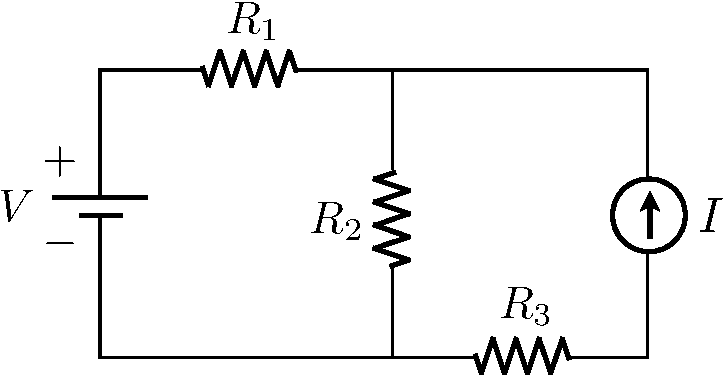
\includegraphics[height=1.25in]{3_fig5_3}}
\caption{Problem \ref{2009_a5_3}.
\label{fig_a5_3}}
\end{figure}
We use loop currents to solve the network depicted in figure \ref{2009_a5_3}.

Kirchhoff's second law gives that $i_2=-I$, and the first law applied to the closed loop on the left gives
$$
R_1i_1+R_2(i_1-i_2)=V.
$$
As $R_1 = 3[\Omega]$, $R_2=1[\Omega]$, $R_3 = 4[\Omega]$, $V=26[V]$, and $I=2[A]$, we get
\begin{eqnarray}
  &&i_2 = -2[A] \\
	&&3i_1+i_1+2=26
\end{eqnarray}
Hence $i_1 = 6[A]$, and from the sign we get that $i_2$ flows in the opposite direction as initially supposed.
\begin{enumerate}[a)]
\item Voltage drop $=R_3i_2=-8[V]$. The - sign indicates that the potential is higher at the left of $R_3$ than on the right.
\item The flow through $R_2$ is $i_1-i_2=8[A]$.
\item Voltage drop $=R_1i_1=18[V]$.
\end{enumerate}



%%%%%%%%%%%%%%%%%%%%%%%%%%%%%%%%%%%%%%%%%%%%%%%%%%%%%%%%%%%%%%%%%%%%%%%%%%%%%%%%
\vspace{2mm}
\noindent {\bf Solution \ref{2009_a5_4}}
Again, we use loop currents to solve the problem depicted in figure \ref{2009_a5_4}.
\begin{figure}
\centerline{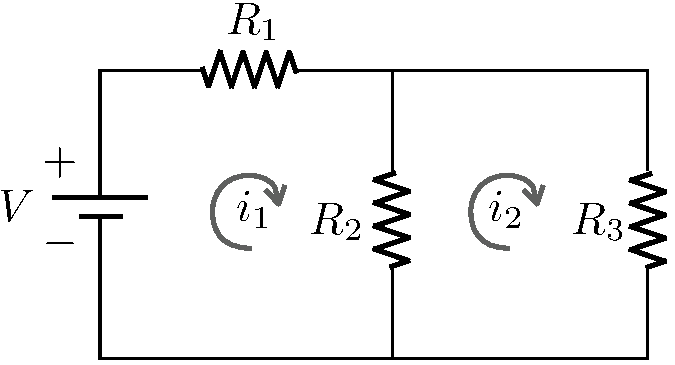
\includegraphics[height=1.25in]{3_fig5_4}}
\caption{Problem \ref{2009_a5_4}.
\label{fig_a5_4}}
\end{figure}

\begin{eqnarray*}
  &&R_1i_1 + R_2(i_1-i_2) = V \\
	&&R_3i_2 + R_2(i_2-i_1) = 0,
\end{eqnarray*}
% 
with $R_1 = 4[\Omega]$, $R_2 = 1[\Omega]$, $R_3 = 2[\Omega]$.

The flow through $R_3$ is $i_2$, which is $1.5[A]$. The system becomes
$$
\left\{\begin{array}{c}4i_1+(i_1-1.5)=V \\ 3+(1.5-i_1)=0 \end{array}\right.
$$
$$
\left\{\begin{array}{c}5i_1-V=\frac{3}{2} \\ i_1=\frac{9}{2} \end{array}\right.
$$
Therefore $V=21[V]$, and $i_1=4.5[A]$
\begin{enumerate}[a)]
\item Voltage drop $=R_3i_2=3[V]$.
\item Current flow $=i_1-i_2=3[A]$.
\item Voltage drop $=V=21[V]$
\end{enumerate}

%%%%%%%%%%%%%%%%%%%%%%%%%%%%%%%%%%%%%%%%%%%%%%%%%%%%%%%%%%%%%%%%%%%%%%%%%%%%%%%%
\vspace{2mm}
\noindent {\bf Solution \ref{2009_a5_5}}
\begin{figure}
\centerline{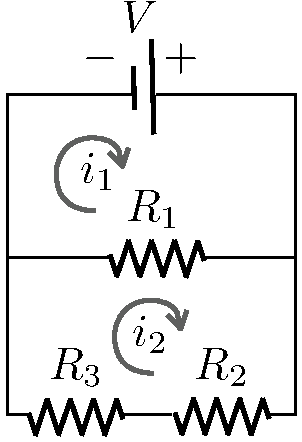
\includegraphics[height=2.25in]{3_fig5_5}}
\caption{Problem \ref{2009_a5_5}.
\label{fig_a5_5}}
\end{figure}
As before:
$$
\left\{\begin{array}{c}R_1(i_1-i_2)=V \\ R_2i_2+R_3i_2+R_1(i_2-i_1)=0 \end{array}\right.,
$$
with $R_1 = 4[\Omega]$, $R_2 = 2[\Omega]$, $R_3 = 10[\Omega]$, $V=60[V]$.

Hence, the system becomes
$$
\left\{\begin{array}{c}4(i_1-i_2)=15 \\ 2i_2+10i_2+4(i_2-i_1)=0 \end{array}\right.,
$$
$$
\left\{\begin{array}{c}i_1-i_2=15 \\ 4i_2-i_1=0 \end{array}\right..
$$
Solving the system we get $i_1 = 20[A]$, $i_2=5[A]$.
\begin{enumerate}[a)]
\item Voltage drop $=R_2i_2=10[V]$.
\item Current flow through $R_1=i_1-i_2=15[A]$.
\item Current flow through $R_3=i_2=5[A]$.
\end{enumerate}

%%%%%%%%%%%%%%%%%%%%%%%%%%%%%%%%%%%%%%%%%%%%%%%%%%%%%%%%%%%%%%%%%%%%%%%%%%%%%%%%
\vspace{2mm}
\noindent {\bf Solution \ref{2009_a6_1}}
Using Kirchhoff's laws we get the following equations:
$$
\left\{\begin{array}{c}R_1i_1+R_2(i_1-i_2)=E_1 \\ R_3i_2+R_2(i_2-i_1)=-E_2\\R_4i_3=E_2 \end{array}\right.,
$$
Plugging in the values of $R_1,R_2,R_3,R_4,E_1$, and $E_2$, we get
$$
\left\{\begin{array}{c}i_1+3(i_1-i_2)=10 \\ 5i_2+3(i_2-i_1)=-4\\2i_3=4 \end{array}\right.,
$$
We have that $i_3=2$. To find $i_1$ and $i_2$ we solve the augmented system
\begin{eqnarray*}
&&\left[\begin{array}{cc|c} 4&-3&10\\-3&8&-4 \end{array}\right]\rarr
\begin{array}{c} (1,:)=(1,:)+(2,:) \end{array}\rarr\\
&&\left[\begin{array}{cc|c} 1&5&6\\-3&8&-4 \end{array}\right]\rarr
\begin{array}{c} (2,:)=(2,:)+3(1,:) \end{array}\rarr
\left[\begin{array}{cc|c} 1&5&6\\0&23&14 \end{array}\right].
\end{eqnarray*}
So $i_1=\frac{68}{23}[A]$, $i_2=\frac{14}{23}[A]$, $i_3=2[A]$.

%%%%%%%%%%%%%%%%%%%%%%%%%%%%%%%%%%%%%%%%%%%%%%%%%%%%%%%%%%%%%%%%%%%%%%%%%%%%%%%%
\vspace{2mm}
\noindent {\bf Solution \ref{2009_a6_2}}
From Kirchhoff's first law:
$$
I+i_3=i_2
$$
From Kirchhoff's second law:
\begin{eqnarray*}
  R_1i_1+R_2(i_1-i_2)=V\\
	E+R_2(i_2-i_1)=0\\
	R_4i_3+R_3i_3=E
\end{eqnarray*}
Substituting in the actual values, we get
$$
\left\{\begin{array}{c}i_1+2 (i_1-i_2)=25\\ i_3-i_2=3\\ E+2(i_2-i_1)=0\\2i_3=E \end{array}\right.
$$
The system, with respect to $i_1,i_2,i_3$, and $E$, yields the following augmented matrix:
\[
\left[\begin{array}{cccc|c} 3 &-2 &0&0&25 \\ 0&-1&1&0&3 \\ -2&2&0&1&0 \\ 0&0&2&-1&0\end{array}\right] \sim 
\left[\begin{array}{cccc|c} 1 & 0 &0&0& 11\\ 0&1&0&0&4 \\ 0&0&1&0&7 \\ 0&0&0&1&14\end{array}\right]
%\\
%&&\rarr \begin{array}{c}(3,:)=(3,:)-(2,:) \end{array}\rarr
%\left[\begin{array}{cccc|c} 2&-1&0&0&25 \\ 0&1&-1&0&3 \\ 0&0&1&1&-3 \\ 0&0&2&-1&0\end{array}\right]
%\rarr \begin{array}{c}(4,:)=(4,:)-2(3,:) \end{array}\rarr\\
%&&\left[\begin{array}{cccc|c} 2&-1&0&0&25 \\ 0&1&-1&0&3 \\ 0&0&1&1&-3 \\ 0&0&0&-3&6\end{array}\right]
\]
\begin{enumerate}[a)]
\item Then $i_1=11[A]$, $i_2=4[A]$, $i_3=7[A]$, $E=14[V]$.
\item Voltage drop (from top to bottom): $R_2(i_1-i_2)=14[V]$. Can also be seen to be the same as $E$. 
\item Current flow through $V$: $i_1=11 [A]$ (upwards).
\end{enumerate}

%%%%%%%%%%%%%%%%%%%%%%%%%%%%%%%%%%%%%%%%%%%%%%%%%%%%%%%%%%%%%%%%%%%%%%%%%%%%%%%%
%\vspace{2mm}
%\noindent {\bf Solution \ref{2009_a6_3}}
%\begin{figure}
%\centerline{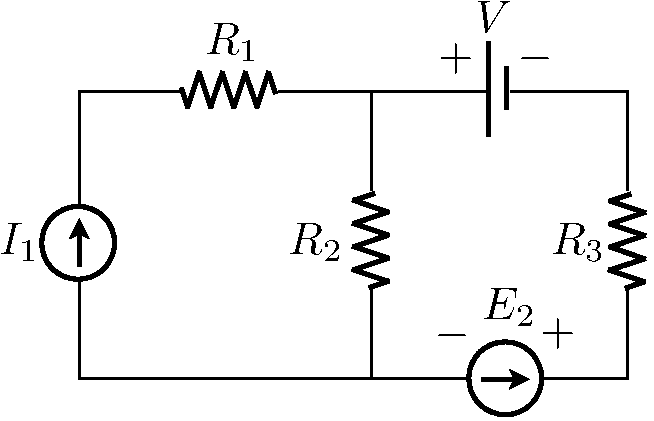
\includegraphics[height=1.5in]{3_fig6_3}}
%\caption{Problem \ref{2009_a6_3}.
%\label{fig_a6_3}}
%\end{figure}
%From Kirchhoff's second law:
%\begin{eqnarray*}
%  I_1=i_1\\
%	I_2=-i_2
%\end{eqnarray*}
%From Kirchhoff's first law:
%\begin{eqnarray*}
%  R_1i_1+R_2(i_1-i_2)=E_1\\
%	V+R_3i_2+E_2+R_2(i_2-i_1)=0,
%\end{eqnarray*}
%which becomes
%$$
%\left\{\begin{array}{c}i_1=I_1\\i_2=-3\\7i_1-5i_2=E_1\\10+8i_2-5i_1+5=0 \end{array}\right.
%$$
%We seek $i_1$ and $E_1$:
%$$
%\left\{\begin{array}{c}7i_1-E_1=-15\\-5i_1=9 \end{array}\right..
%$$
%Therefore we have that $i_1 = -\frac{9}{5}[A]$, $E_1=\frac{12}{5}[V]$.
%\begin{enumerate}[a)]
%\item Current flow through $R_2$: $i_1-i_2=\frac{6}{5}[A]$.
%\item Voltage drop through $I_1=E_1=\frac{12}{5}[V]$.
%\item Current flow through $I_1=i_1=-\frac{9}{5}[A]$.
%\end{enumerate}

%%%%%%%%%%%%%%%%%%%%%%%%%%%%%%%%%%%%%%%%%%%%%%%%%%%%%%%%%%%%%%%%%%%%%%%%%%%%%%%%
\vspace{2mm}
\noindent {\bf Solution \ref{op2_17}}
Note that this solution follows the alternate description of resistor 
networks in the notes. 
Using the identities $V_i=I_iR_i$, the voltage equations for the loops 
can be written
\begin{eqnarray*}
I_1R_1 + I_2R_2 + E &= &0 \\
I_3R_3 + I_4R_4 - I_2R_2 &= & 0 \\
&\vdots &  \\
I_{2n-1}R_{2n-1} + I_{2n}R_{2n} - I_{2n-2}R_{2n-2} &= &0
\end{eqnarray*}
The current equations for the nodes are 
\begin{eqnarray*}
I_1-I_3-I_2&=&0 \\
I_3-I_5-I_4&=&0 \\
&\vdots& \\
I_{2n-1}-I_{2n}&=&0 \\
\end{eqnarray*}

%%%%%%%%%%%%%%%%%%%%%%%%%%%%%%%%%%%%%%%%%%%%%%%%%%%%%%%%%%%%%%%%%%%%%%%%%%%%%%%%
\vspace{2mm}
\noindent {\bf Solution \ref{op2_13}}
We have $n=6$, $\sum x_i=15$, $\sum x_i^2=43$, $\sum y_i=18$,
$\sum x_iy_i=52$, so $a=14/11\sim 1.27\ldots$ and $b=-2/11\sim-0.18\ldots$.
%The solution is shown in Figure~\ref{fig_lsq}.
%
%\begin{figure}
%\centerline{\includegraphics[height=1.5in]{lsq}}
%\caption{Least squares fit of Solution~\ref{op2_13}.
%\label{fig_lsq}}
%\end{figure}

%%%%%%%%%%%%%%%%%%%%%%%%%%%%%%%%%%%%%%%%%%%%%%%%%%%%%%%%%%%%%%%%%%%%%%%%%%%%%%%%
\vspace{2mm}
\noindent {\bf Solution \ref{op2_14}}
We would want to minimize the quadratic function
\begin{eqnarray*}
f(a,b,c)&=&\sum(ax_i^2+bx_i+c-y_i)^2 \\
&=& \sum
\left(	a^2x_i^4 	+ b^2x_i^2 	+ c^2+y_i^2 	+ 2abx_i^3
	+2acx_i^2	-2ax_i^2y_i	+2bcx_i		-2bx_iy_i 	-2cy_i
	\right) \\
&=& \left(\sum x_i^4\right)a^2
+\left(\sum x_i^2\right)b^2
+nc^2
+2\left(\sum x_i^3\right)ab
+2\left(\sum x_i^2\right)ac
+2\left(\sum x_i\right)bc \\
& & 
-2\left(\sum x_i^2y_i\right)a
-2\left(\sum x_iy_i\right)b
-2\left(\sum y_i\right)c
+\left(\sum y_i^2\right)
\end{eqnarray*}
The corresponding system of equations is
\[
\left[\matrix{
\left(\sum x_i^4\right)&\left(\sum x_i^3\right)&\left(\sum x_i^2\right)\cr
\left(\sum x_i^3\right)&\left(\sum x_i^2\right)&\left(\sum x_i\right)\cr
\left(\sum x_i^2\right)&\left(\sum x_i\right)&n\cr
}\right.\left|\matrix{
\left(\sum x_i^2y_i\right)\cr \left(\sum x_iy_i\right)
\cr \left(\sum y_i\right)\cr
}\right]
\]
(I've divided each equation by two.)

%%%%%%%%%%%%%%%%%%%%%%%%%%%%%%%%%%%%%%%%%%%%%%%%%%%%%%%%%%%%%%%%%%%%%%%%%%%%%%%%
\vspace{2mm}
\noindent {\bf Solution \ref{op2_15}}
The matrix is
\[
\left[\matrix{
k_1+k_2	&-k2	&0	&0	&\ldots	&0	&0	&0\cr
-k_2	&k_2+k_3&-k_3	&0	&\ldots	&0	&0	&0\cr
0	&-k_3	&k_3+k_4&-k_4	&\ldots	&0	&0	&0\cr
0	&0	&-k_4	&k_4+k_5&\ldots	&0	&0	&0\cr
0	&0	&0	&-k_5	&\ldots	&0	&0	&0\cr
\vdots	&\vdots	&\vdots	&\vdots	&	&\vdots	&\vdots	&\vdots\cr
0	&0	&0	&0	&\ldots	&-k_{n-1}&k_{n-1}+k_n&-k_n\cr
0	&0	&0	&0	&\ldots	&0	&-k_n	&k_n\cr
}\right.\left|\matrix{
m_1g +k_1 l_1 - k_2 l_2\cr
m_2g +k_2 l_2 - k_3 l_3 \cr
m_3g +k_3 l_3 - k_4 l_4 \cr
m_4g +k_4 l_4 - k_5 l_5 \cr
m_5g +k_5 l_5 - k_6 l_6 \cr
\vdots\cr
m_{n-1}g +k_{n-1} l_{n-1} - k_{n} l_{n} \cr
m_g +k_n l_n\cr
}\right]
\]

%%%%%%%%%%%%%%%%%%%%%%%%%%%%%%%%%%%%%%%%%%%%%%%%%%%%%%%%%%%%%%%%%%%%%%%%%%%%%%%%
\vspace{2mm}
\noindent {\bf Solution \ref{op2_16}}
The system of equations would be
\[
\left[\matrix{
2&-1&0&0&0\cr
-1&2&-1&0&0\cr
0&-1&2&-1&0\cr
0&0&-1&2&-1\cr
0&0&0&-1&1\cr
}\right.\left|\matrix{\
g\cr 2g\cr 3g\cr 4g\cr 5g+1\cr
}\right]
\]


% \end{document}
